\chapter{ColPali Appendix}

\section*{Reproducibility Statement}

For transparency, reproducibility and to foster future work, we release our training data, model checkpoints (adapters), entire codebase, and complete evaluation benchmark under MIT licenses as detailed in the main paper. We also host a public \textsc{ViDoRe} leaderboard\sidenote{\url{https://huggingface.co/spaces/vidore/vidore-leaderboard}} to foster concurrent work in the space. The supplementary material further details training configurations for our models (also specified in HuggingFace model repositories), and dives into the process we used to generate synthetic data, how latency computations are performed, as well as provides further detailed evaluation results.



\section*{Acknowledgements}

This work is partially supported by Illuin Technology, and by a grant from ANRT France. This work was performed using HPC resources from the CINES ADASTRA through Grant 2024-AD011015443 and from IDRIS with grant 2024-AD011015724R1.
We extend our warm thanks to Jonathan Dong, Caio Corro, Victor Pellegrain and Ender Konukoglu for their valuable feedback on the paper.


\section{Benchmark Datasets}

\subsection{Academic Datasets}
\label{subsection:academic_datasets}

\noindent\textbf{DocVQA} \sidecite{mathew_docvqa_2020} includes collected images from the UCSF Industry Documents Library. Questions and answers were manually annotated.

\noindent\textbf{InfoVQA} \sidecite{mathew_infographicvqa_2021} includes infographics collected from the Internet using the search query “\textit{infographics}”. Questions and answers were manually annotated.

\noindent\textbf{TAT-DQA} \sidecite{zhu_towards_2022} is a large-scale Document VQA dataset that was constructed from publicly available real-world financial reports. It focuses on rich tabular and textual content requiring numerical reasoning. Questions and answers were manually annotated by human experts in finance.

\noindent\textbf{arXivQA} \sidecite{li2024multimodal} is a VQA dataset based on figures extracted from arXiv publications. The questions were generated synthetically using GPT-4 Vision.

\noindent\textbf{TabFQuAD} (Table French Question Answering Dataset) is designed to evaluate TableQA models in realistic industry settings. We create additional queries to augment the existing human-annotated ones using the same method described in \autoref{subsection:docvisbench_methodology}.

\label{subsection:tabfquad}
% create new queries following the same methodology as in\autoref{paragraph:query_generation} but with GPT-4 Vision. Eventually, we obtained a retrieval version of TabFQuAD with 1,800 document query pairs, which we split into a training set of 1550 examples and a test set of 250 examples.


\subsection{Practical Datasets}
\label{subsection:docvisbench_methodology}
%Hugging Face collection: \url{https://huggingface.co/collections/coldoc/syntheticdocqa-test-6655c59cfda461267c0d9ac8}

% \subsubsection{Method}

\noindent\textbf{Methodology.} Creating a relevant retrieval dataset close to real use cases is a major challenge as the dataset needs to be both sufficiently large for effective fine-tuning and sufficiently diverse to cover a broad range of modalities (full text, tables, charts, ...), domains (industry, healthcare, ...), and query-document interactions (extractive questions, open-ended questions, ...). Our approach to building this dataset involves several steps: (1) we use a web crawler to collect publicly available documents on various themes and sources, (2) we convert these PDFs into a series of images, one per page, and (3) we generate queries related to each image using a VLM.

\noindent\textbf{Web-Crawler.} We implemented a web crawler to efficiently collect large volumes of documents related to a given topic. The crawler is seeded with a user-defined query (e.g.\ ``artificial intelligence") and then uses GPT-3.5 Turbo to brainstorm related topics and subtopics. This query augmentation strategy aims at both broadening and deepening the search. GPT-3.5 Turbo is further used to generate diverse search queries from each subtopic. This query set is then consumed by a pool of parallel workers whose job is to fetch the associated most relevant documents. We use SerpAPI\sidenote{\url{https://serpapi.com/}} along with a filetype filter (PDF documents only) to programmatically scrape Google Search rankings. Each file is hashed and stored in a Bloom filter \sidecite{bloom_spacetime_1970} shared among workers to avoid duplicate documents in the final corpus. Unique scraped files are downloaded, and inserted into a SQLite database along with additional metadata.

\noindent\textbf{Datamix.} Using the web crawler, we collected approximately 100 documents for each of the following four seeds: \textit{``energy"}, \textit{``government reports"}, \textit{``healthcare industry"}, and \textit{``artificial intelligence"}. These seeds were meticulously hand-picked to align with real-use cases for retrieval models and visually rich pages. We also removed all documents containing any private information. 

\noindent\textbf{Query Generation.}\label{paragraph:query_generation} To increase the efficiency of our query generation scheme and to limit API calls, we generate at most 3 questions per image. From all the documents collected, we randomly sample 10,000 images per theme and call Claude-3 Sonnet with the following prompt:


\begin{kaobox}

You are an assistant specialized in Multimodal RAG tasks.

The task is the following: given an image from a pdf page, you will have to 
generate questions that can be asked by a user to retrieve information from 
a large documentary corpus. 
The question should be relevant to the page, and should not be too specific 
or too general. The question should be about the subject of the page, and 
the answer needs to be found in the page.

Remember that the question is asked by a user to get some information from a
large documentary corpus that contains multimodal data. Generate a question 
that could be asked by a user without knowing the existence and the content 
of the corpus.
Generate as well the answer to the question, which should be found in the
page. And the format of the answer should be a list of words answering the
question.
Generate at most THREE pairs of questions and answers per page in a dictionary
with the following format, answer ONLY this dictionary NOTHING ELSE:

{
    "questions": [
        {
            "question": "XXXXXX",
            "answer": ["YYYYYY"]
        },
        {
            "question": "XXXXXX",
            "answer": ["YYYYYY"]
        },
        {
            "question": "XXXXXX",
            "answer": ["YYYYYY"]
        },
    ]
}
where XXXXXX is the question and ['YYYYYY'] is the corresponding list of answers
that could be as long as needed.

Note: If there are no questions to ask about the page, return an empty list.
Focus on making relevant questions concerning the page.
Here is the page:

\end{kaobox}

% \subsection{TabFQuAD}
% \label{subsection:tabfquad}
% \noindent\textbf{Data Collection.} TabFQuAD (Table French Question Answering Dataset) is designed to evaluate TableQA models in realistic industry settings. TabFQuAD is created by: (1) using an internet scrapper to retrieve PDF documents from the websites of large companies and government agencies (2) using a custom table extraction pipeline based on both manual heuristics and deep learning methods to detect \sidecite{huang_layoutlmv3_2022} and reconstruct \sidecite{qiao_lgpma_2021} tables from the original PDF documents, and (3) manually inspecting each table and filter out low-quality extractions. In the end, we obtain 2,308 industry-realistic tables from a wide range of sources. While this process was designed to automate a large part of the work, we believe having a human evaluation step was required to ensure high-quality data that does not propagate errors from the extraction pipeline.

% \begin{figure}
%     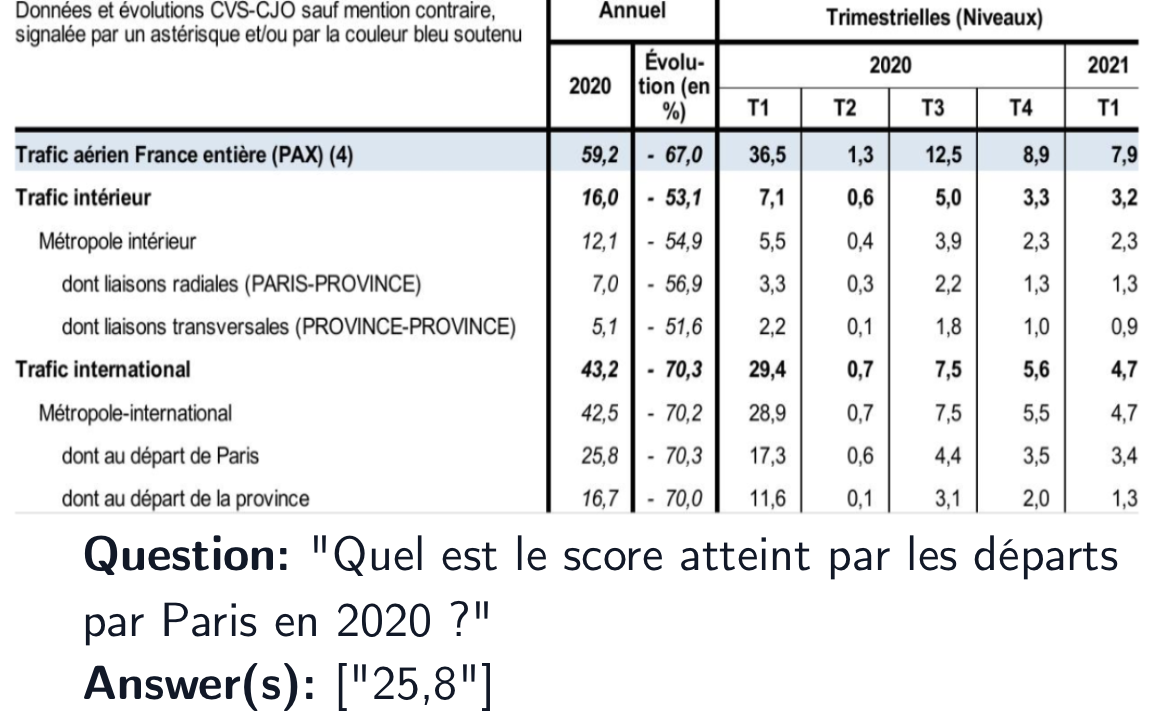
\includegraphics[width=0.45\textwidth]{images/colpali_images/dataset_samples/tabfquad_example.png}
%     \caption{TabFQuAD contains visually rich tables, e.g. this example with highlighted numbers, cell background, and custom cell lines for delimiting subcategories.}
% \end{figure}

% \noindent\textbf{Integration in \textit{ViDoRe}.}
% For our use case, we used the test set of TabFQuAD by filtering out adversarial questions as we are interested in a retrieval task.
% In the original TabFQuAD dataset, we observed that certain questions are irrelevant to the retrieval task. For instance, \textit{When was the project created?} (in French, \textit{Quand a été crée le projet ?}) is too vague. Thus, we have decided to keep the table images but to create new queries following the same methodology as in\autoref{paragraph:query_generation} but with GPT-4 Vision. Eventually, we obtained a retrieval version of TabFQuAD with 1,800 document query pairs, which we split into a training set of 1550 examples and a test set of 250 examples.

\noindent\textbf{Human Validation.} We manually validate every single synthetically created query in \textsc{ViDoRe} to ensure quality, query relevance, and consistency with the benchmark objective of evaluating retrieval in practical industrial settings. During this step, we randomly assign document-pair queries to 4 volunteer annotators and instruct them to filter out queries that do not fit the above-listed criteria. We also instruct annotators to flag any documents they deem to contain PII information or content not suited for an academic benchmark. No flag was raised during the entirety of the process, validating our prior PDF collection strategy. 100 queries per topic are collected in this manner. Annotators are colleagues and collaborators of the authors who volunteered to help. Each annotator spent approximately 3 hours filtering the larger query set down to 100 high-quality queries per topic.

\subsection{Training Dataset}
\label{subsection:training_dataset}
The statistics of the train set are given in the following table. The creation of the train set follows the same methodology as in \autoref{subsection:docvisbench_methodology}. We made sure that a PDF document cannot have pages in both the training set and the test set to prevent data leakage and that there are no duplicate documents in each split.

\begin{table}[ht]
    \centering
    \label{tab:datasets}
    \small
    \begin{tabular}{llll}
        \toprule
        \textbf{Dataset Split} & \textbf{Split Size} & \textbf{Language} & \textbf{Domain}\\
        \midrule
        DocVQA & 39,463 & English & Scanned documents from UCSF Industry\\
        InfoVQA & 10,074 & English & Infographics scraped from the web \\
        TATDQA & 13,251 & English & High-quality financial reports \\
        arXivQA & 10,000 & English & Scientific Scientific Figures from arXiv\\
        Scraped PDFs & 45,940 & English & Varied PDFs from 3885 distinct URL domains\\
        \midrule
        \textbf{TOTAL} & \textbf{118,695} & \textbf{English-only} & \textbf{Mixed} \\
        \bottomrule
    \end{tabular}
    \caption[ColPali dataset splits]{Details on the different splits in the dataset used to train ColPali.}
    \label{table:training_set_overview}
\end{table}
% \newpage



\section{Implementation details}

\subsection{Codebase}
The codebase is written in PyTorch\sidenote{\url{https://pytorch.org/}} and leverages HuggingFace tooling for model implementations and trainers\sidenote{\url{https://huggingface.co}}.


\subsection{Hyperparameters}

Hyperparameters are tuned on a validation split composed of $2\%$ of the training dataset. We find bi-encoder methods to be more sensible to learning rate variations than late interaction-based models and achieve the best performance for all models with a learning rate of $5e-5$. We experiment with LoRA rank and $\alpha$ values and do not notice particular improvements past $r = \alpha = 32$. Per-device batch sizes are kept small due to long sequence lengths that complicate scaling past $b=4$. We simulate larger batch sizes with multi-GPU training and train with a total batch size $b=32$ with no accumulation, for 1 epoch on our training set.


\subsection{Embedding size}
\label{subsection:embedding_size}

Minimizing storage footprint can be essential to industrial retrieval systems if databases contain millions of documents. With this criterion in view, we have compared the embedding sizes of the models in our study. As shown in \autoref{table:embedding_size}, \textit{ColPali}’s embedding size is an order of magnitude larger than BM25 and two orders of magnitude larger than BGE-M3. However, in practical scenarios, pooling multi-vector embeddings by centroid cluster, or quantizing embeddings to binary representations \sidenote{\url{https://blog.vespa.ai/scaling-colpali-to-billions/}} can reduce storage costs by two orders of magnitude \sidecite{santhanam_plaid_2022} with minimal performance hits, and make storage costs competitive with other systems.

\begin{table}[ht]
    \centering
    \begin{tabular}{l|c}
    % \hline
    \textbf{Model}              & \textbf{Embedding size (KB)} \\
    \hline
    BGE-M3             & 8.60               \\
    BM25 (dense emb.)  & 3.00                \\
    BM25 (sparse emb.) & 1.56 ± 0.51         \\
    \textit{ColPali} (float16)            & 257.5              \\
    % \hline
    \end{tabular}
    \caption[DocVQA embedding sizes]{Comparison of the embedding sizes for the DocVQA test set from \textsc{ViDoRe} w.r.t. different retrieval models. The \textit{mean ± std} size is given for the sparse embeddings. In general multiple vectors (2-5) per page are used for BGE-M3 and BM25.}
    \label{table:embedding_size}
\end{table}


\subsection{Latency computations}
\label{paragraph:latency_app} 
To ensure comparison fairness, the latencies of the different retrieval systems shown in \autoref{fig:latency-comparison} are measured on the same \texttt{g2-standard-8} GCP VM with an NVIDIA L4 GPU. Document pages are embedded using the highest settings of \texttt{Unstructured} with captioning (see \autoref{subsection:baseline_models}). SigLIP and \textit{ColPali} are both loaded with \texttt{bfloat16} parameter dtypes. The reported times in \autoref{table:latency-comparison} are the average per-page latencies for each indexing operation on 1000 randomly chosen documents across all splits of the \textsc{ViDoRe} benchmark test set. A batch size of $8$ was used for the BGE-M3 model used with \texttt{Unstructured}, and a batch size of $4$ was used for SigLIP and \textit{ColPali}.

\begin{table}[ht]
    \centering
    \begin{tabular}{l|c|c|c}
    \multirow{2}{*}{\textbf{Indexing operation}} & \multicolumn{3}{c}{\textbf{Latency (s)}}                                                                      \\ \cline{2-4} 
                                                 & \multicolumn{1}{l|}{\textbf{Unstructured}} & \multicolumn{1}{l|}{\textbf{SigLIP}} & \textit{\textbf{ColPali}} \\
    \hline
    Layout detection                             & \multicolumn{1}{c|}{0.81}                  & \multicolumn{1}{c|}{NA}              & NA                                            \\
    OCR                                          & \multicolumn{1}{c|}{2.67}                  & \multicolumn{1}{c|}{NA}              & NA                                            \\
    Captioning                                   & \multicolumn{1}{c|}{3.71}                  & \multicolumn{1}{c|}{NA}              & NA                                            \\
    Page encoding                                & \multicolumn{1}{c|}{0.03}                  & \multicolumn{1}{c|}{0.12}            & 0.39                                          \\ \hline
    Total                                        & \multicolumn{1}{c|}{7.22}                  & \multicolumn{1}{c|}{0.12}            & 0.39
    \end{tabular}
    \caption[Page-level indexing latencies]{Page-level latencies for document indexing using various retrieval systems. SigLIP and \textit{ColPali} are much faster than \texttt{Unstructured} because they don't require the layout detection, OCR, and captioning operations.}
    \label{table:latency-comparison}
\end{table}


\subsection{Captioning}
\label{paragraph:captioning} 

Examples of captions generated for visually rich document chunks with Claude-3 Sonnet are shown in \autoref{fig:caption_table} and \autoref{fig:caption_figure}. The prompt used for generating the description is the following:

\begin{kaobox}
\small
You are an assistant specialized in document analysis. Given a table or a figure, you have to provide a detailed summary of the content in maximum 3000 characters. Your summary should be qualitative and not quantitative. Here is the table/figure to analyze: \{image\}. Answer ONLY with the caption of the table/figure.
\end{kaobox}

\begin{figure}[ht]
    \centering
    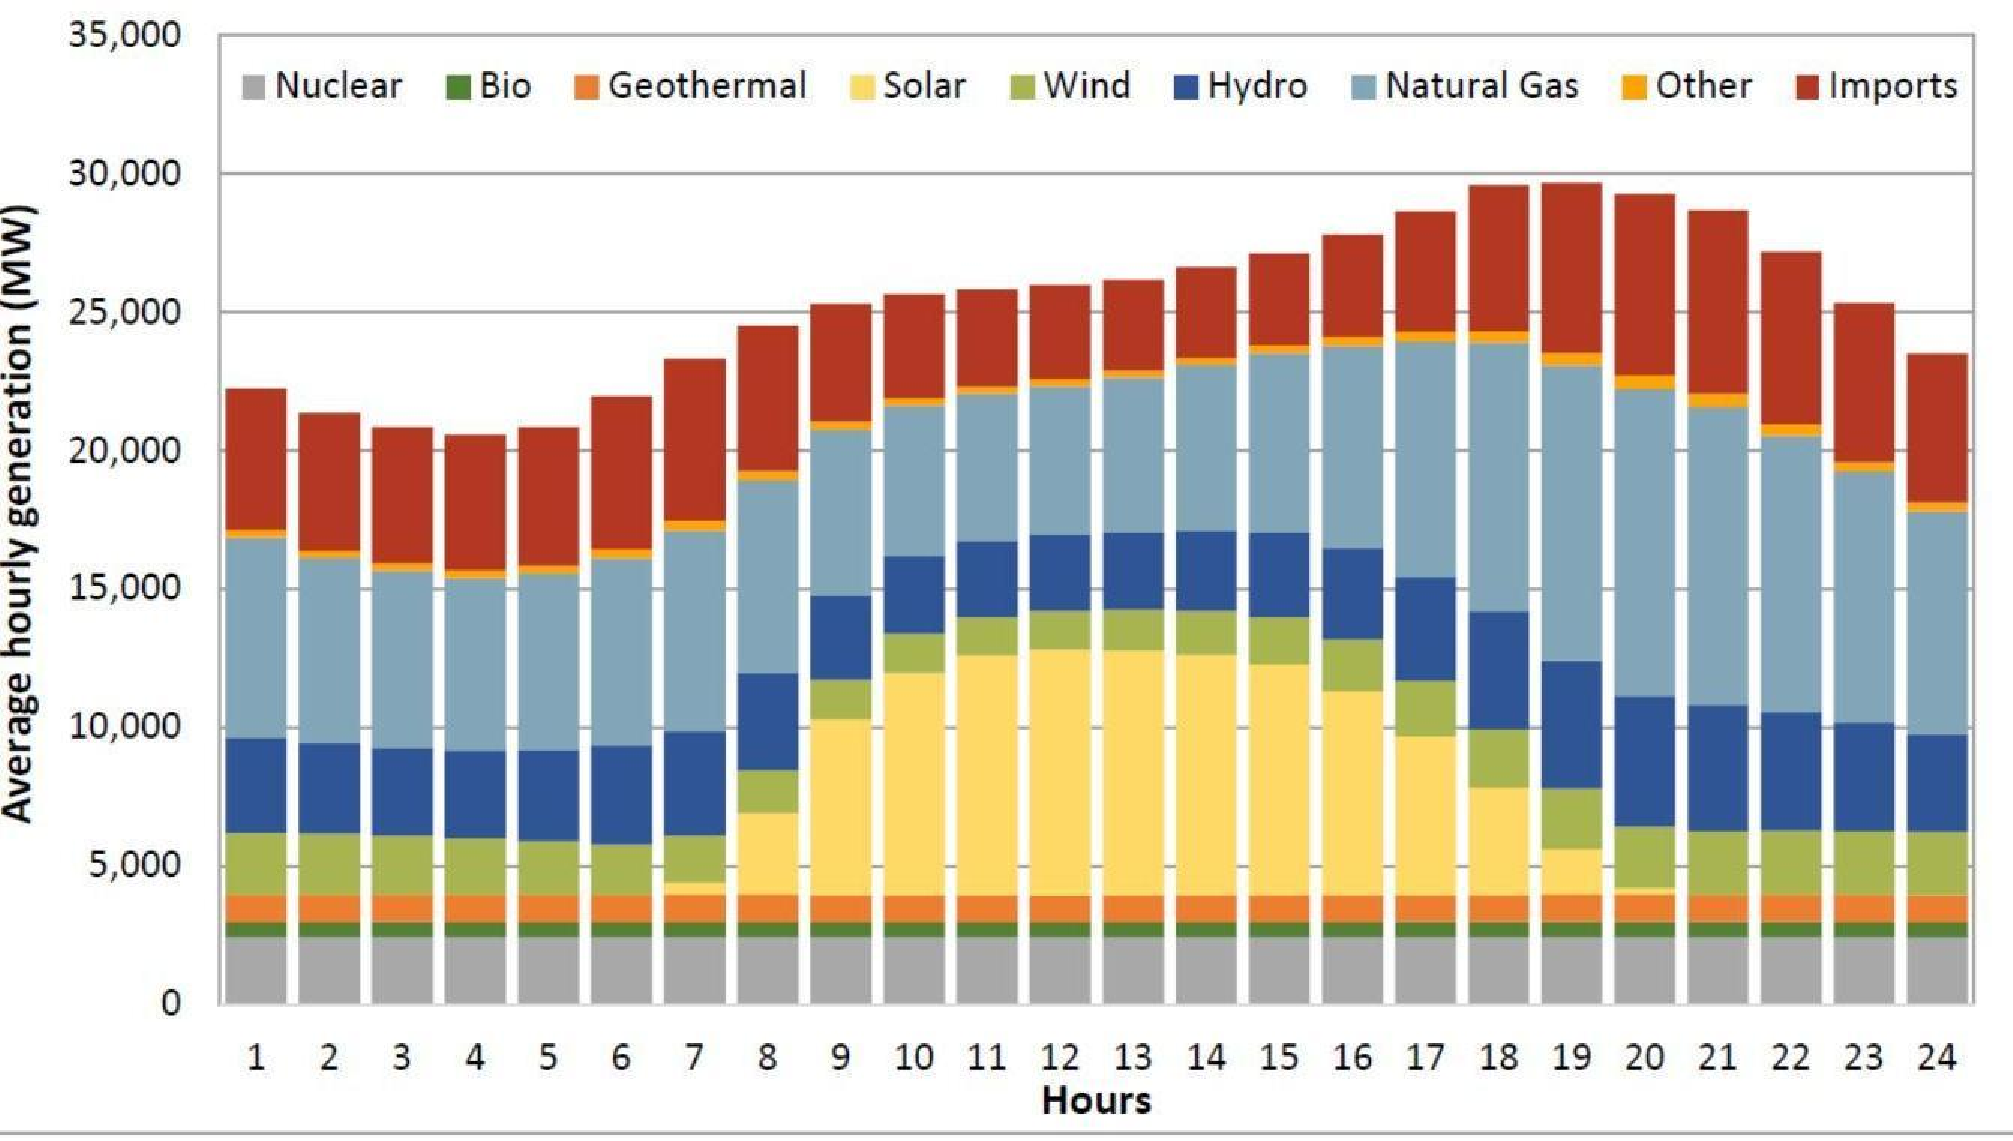
\includegraphics[width = 0.7 \textwidth]{images/colpali_images/ex_figure_caption.pdf}
    
    \caption[Energy test set example]{Example from the ``Energy" test set.\\
    \textbf{Caption:} \textit{The image depicts the hourly energy generation profile, illustrating the contributions of various energy sources over 24 hours. The data is presented as a stacked bar chart, with the x-axis representing the hours of the day from 1 to 2, and the y-axis showing the average hourly generation in MW. The bars are segmented into different colors, each representing a distinct energy source: nuclear, bio, geothermal, solar, wind, hydro, natural gas, and other imports. The chart provides insights into the temporal variations in energy generation across different sources, highlighting the interplay between baseload and intermittent sources throughout the day.}}
    \label{fig:caption_figure}
\end{figure}

% Table to do 

\begin{figure}[ht]
    \centering
    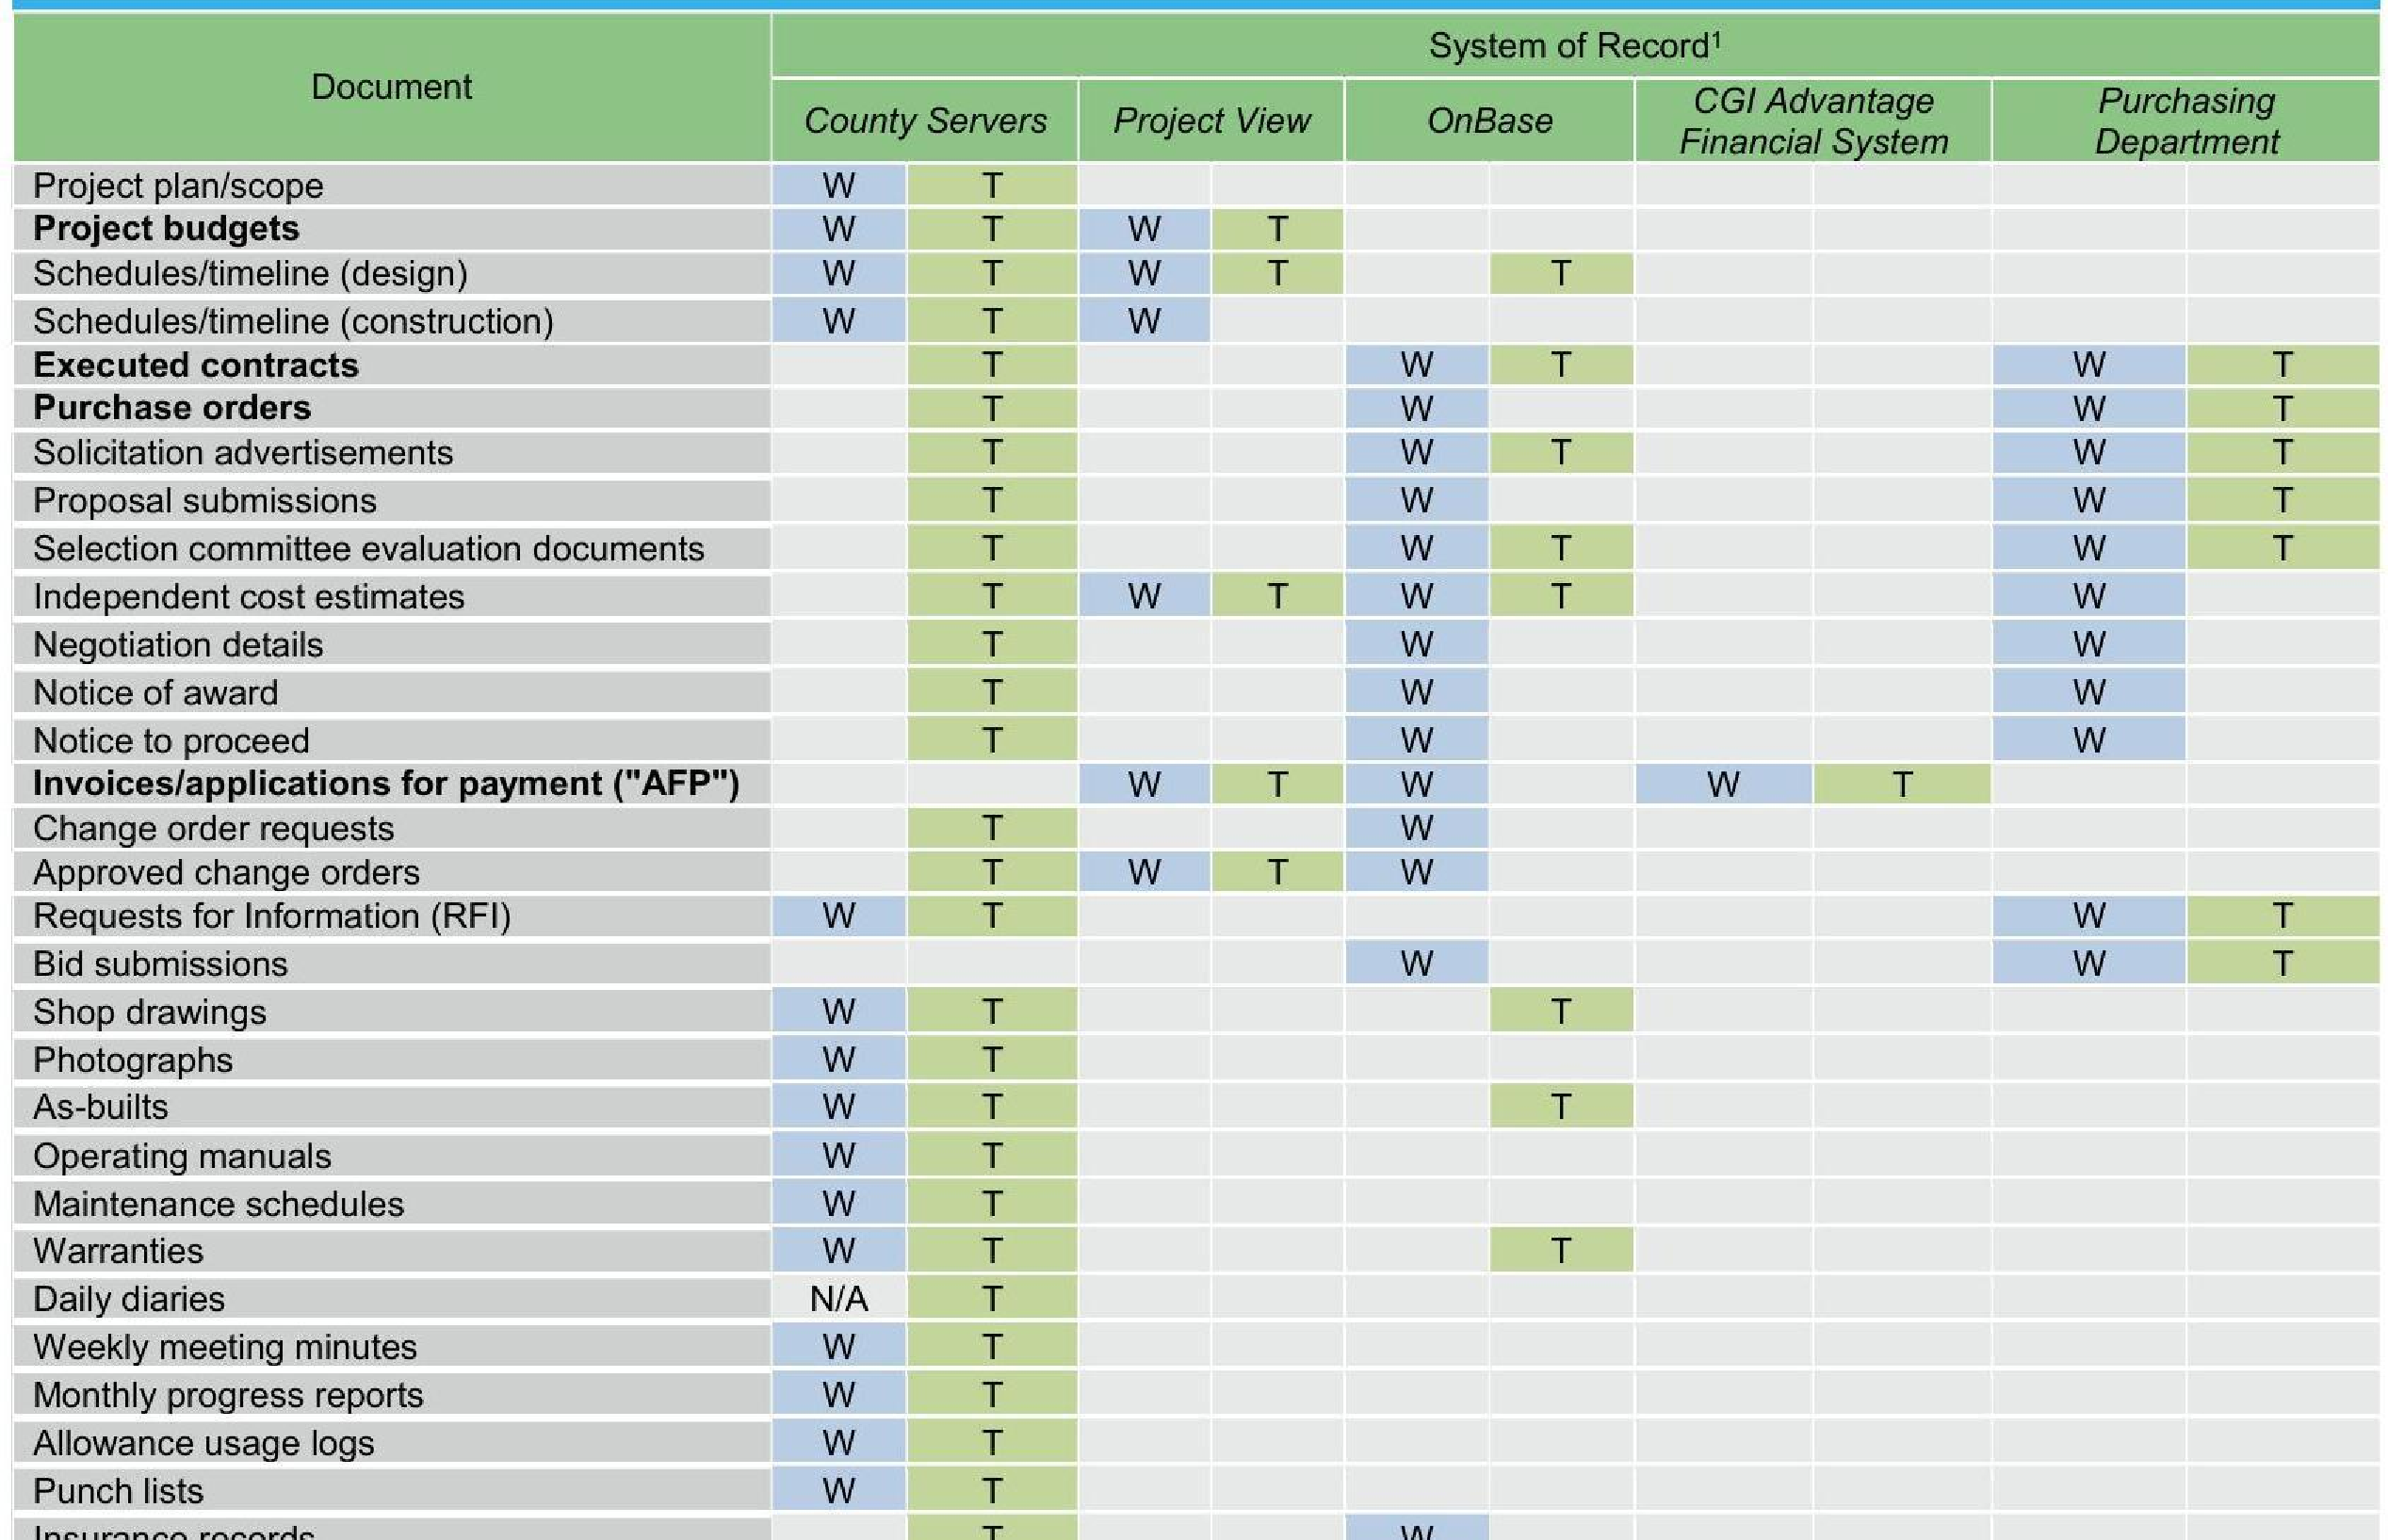
\includegraphics[width = 0.7 \textwidth]{images/colpali_images/ex_table_caption.pdf}
    
    \caption[Government reports example]{Example from the ``Government Reports" test set.\\
    \textbf{Caption:} \textit{The image shows a table titled ``System of Record" which outlines the different types of documents or records maintained across various systems or departments within an organization related to project management and construction. The rows list documents like project plans, budgets, schedules, contracts, purchase orders, invoices, change requests, bid submissions, drawings, manuals, meeting minutes, and reports. The columns indicate the system or department responsible for maintaining each record, such as County Servers, Project View, OnBase, CGI Advantage Financial System, and Purchasing Department. The table uses "W" and "T" markers to denote which system or department serves as the primary source (writer) or storage location (trailer) for each type of document.}}
    \label{fig:caption_table}
\end{figure}



% \newpage
% \section{More similarity maps}
% \label{section:more_similarity_maps}
% In \autoref{fig:similarity_map_kazakhstan}, \textit{ColPali} assigns a high similarity to all patches with the word \textit{"Kazakhstan"} when given the token \texttt{<\_Kazakhstan>}. Moreover, our model seems to exhibit world knowledge capabilities as the patch around the word \textit{"Kashagan"} - an offshore oil field in Kazakhstan - also shows a high similarity score. On the other hand, in \autoref{fig:similarity_map_ferroelectrics}, we observe that \textit{ColPali} is also capable of complex image understanding. Not only are the patches containing the word \textit{"formulations"} highly similar to the query token \texttt{\_formula}, but so is the upper-left molecule structure.

% \begin{figure}
% \centering
%     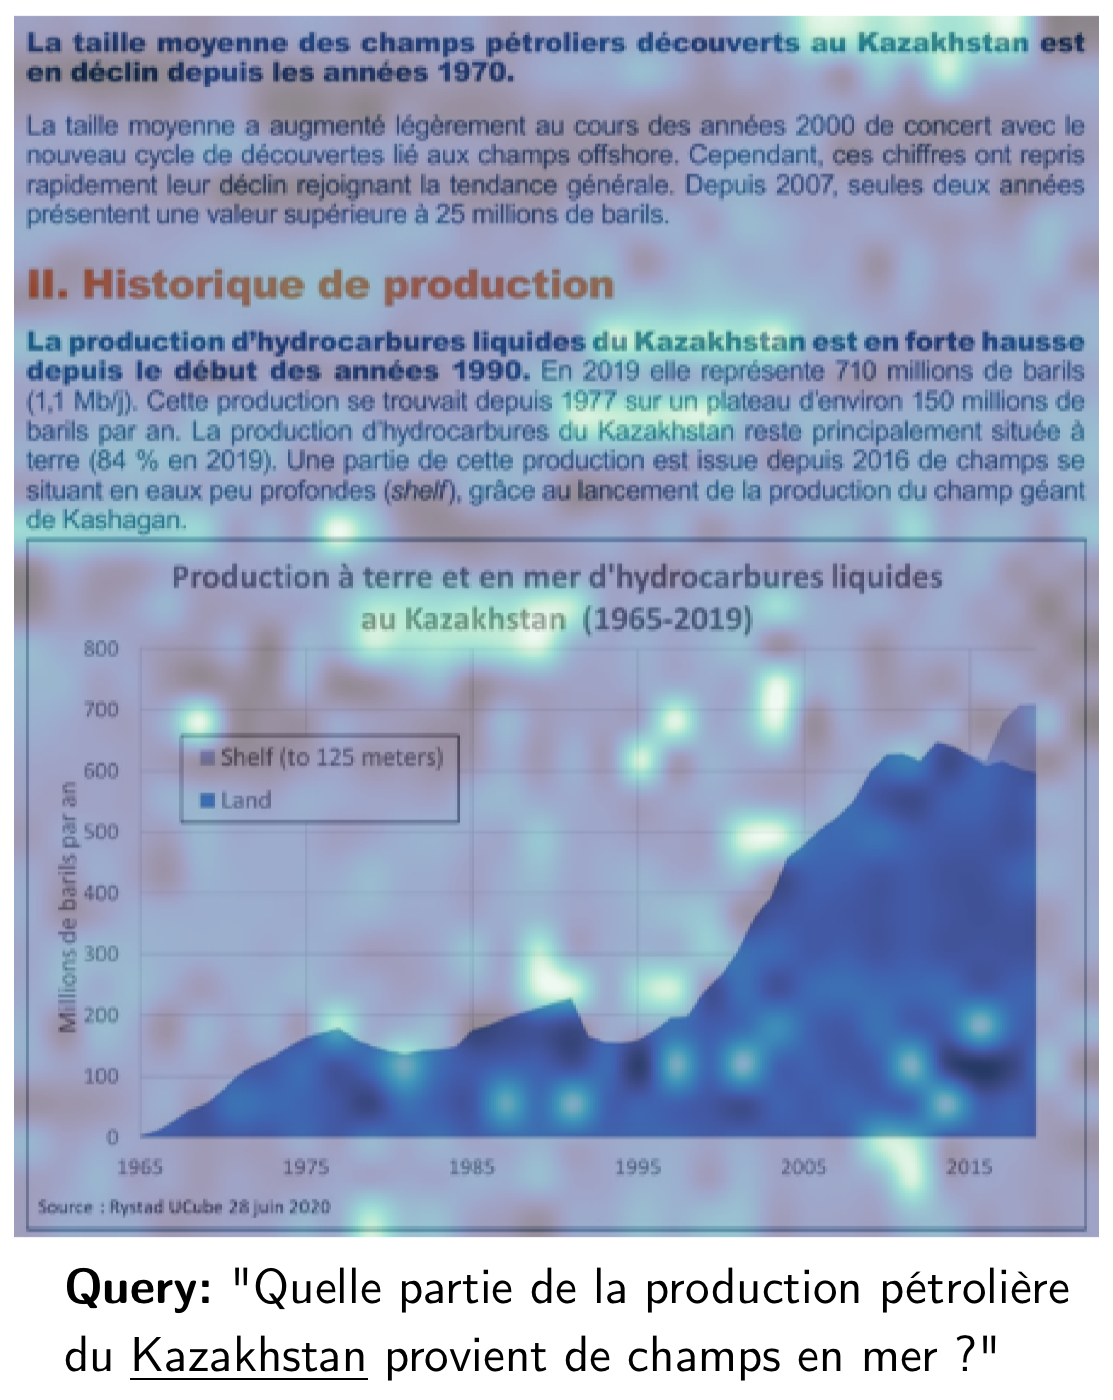
\includegraphics[width=0.8\linewidth]{images/colpali_images/similarity_maps/similarity_map_kazakhstan.png} 
%     \caption{Similarity of the image patches w.r.t. the underlined token in the user query. This example is from the \textit{Shift} test set.}
% \label{fig:similarity_map_kazakhstan}
% \end{figure}

% \begin{figure}
% \centering
% 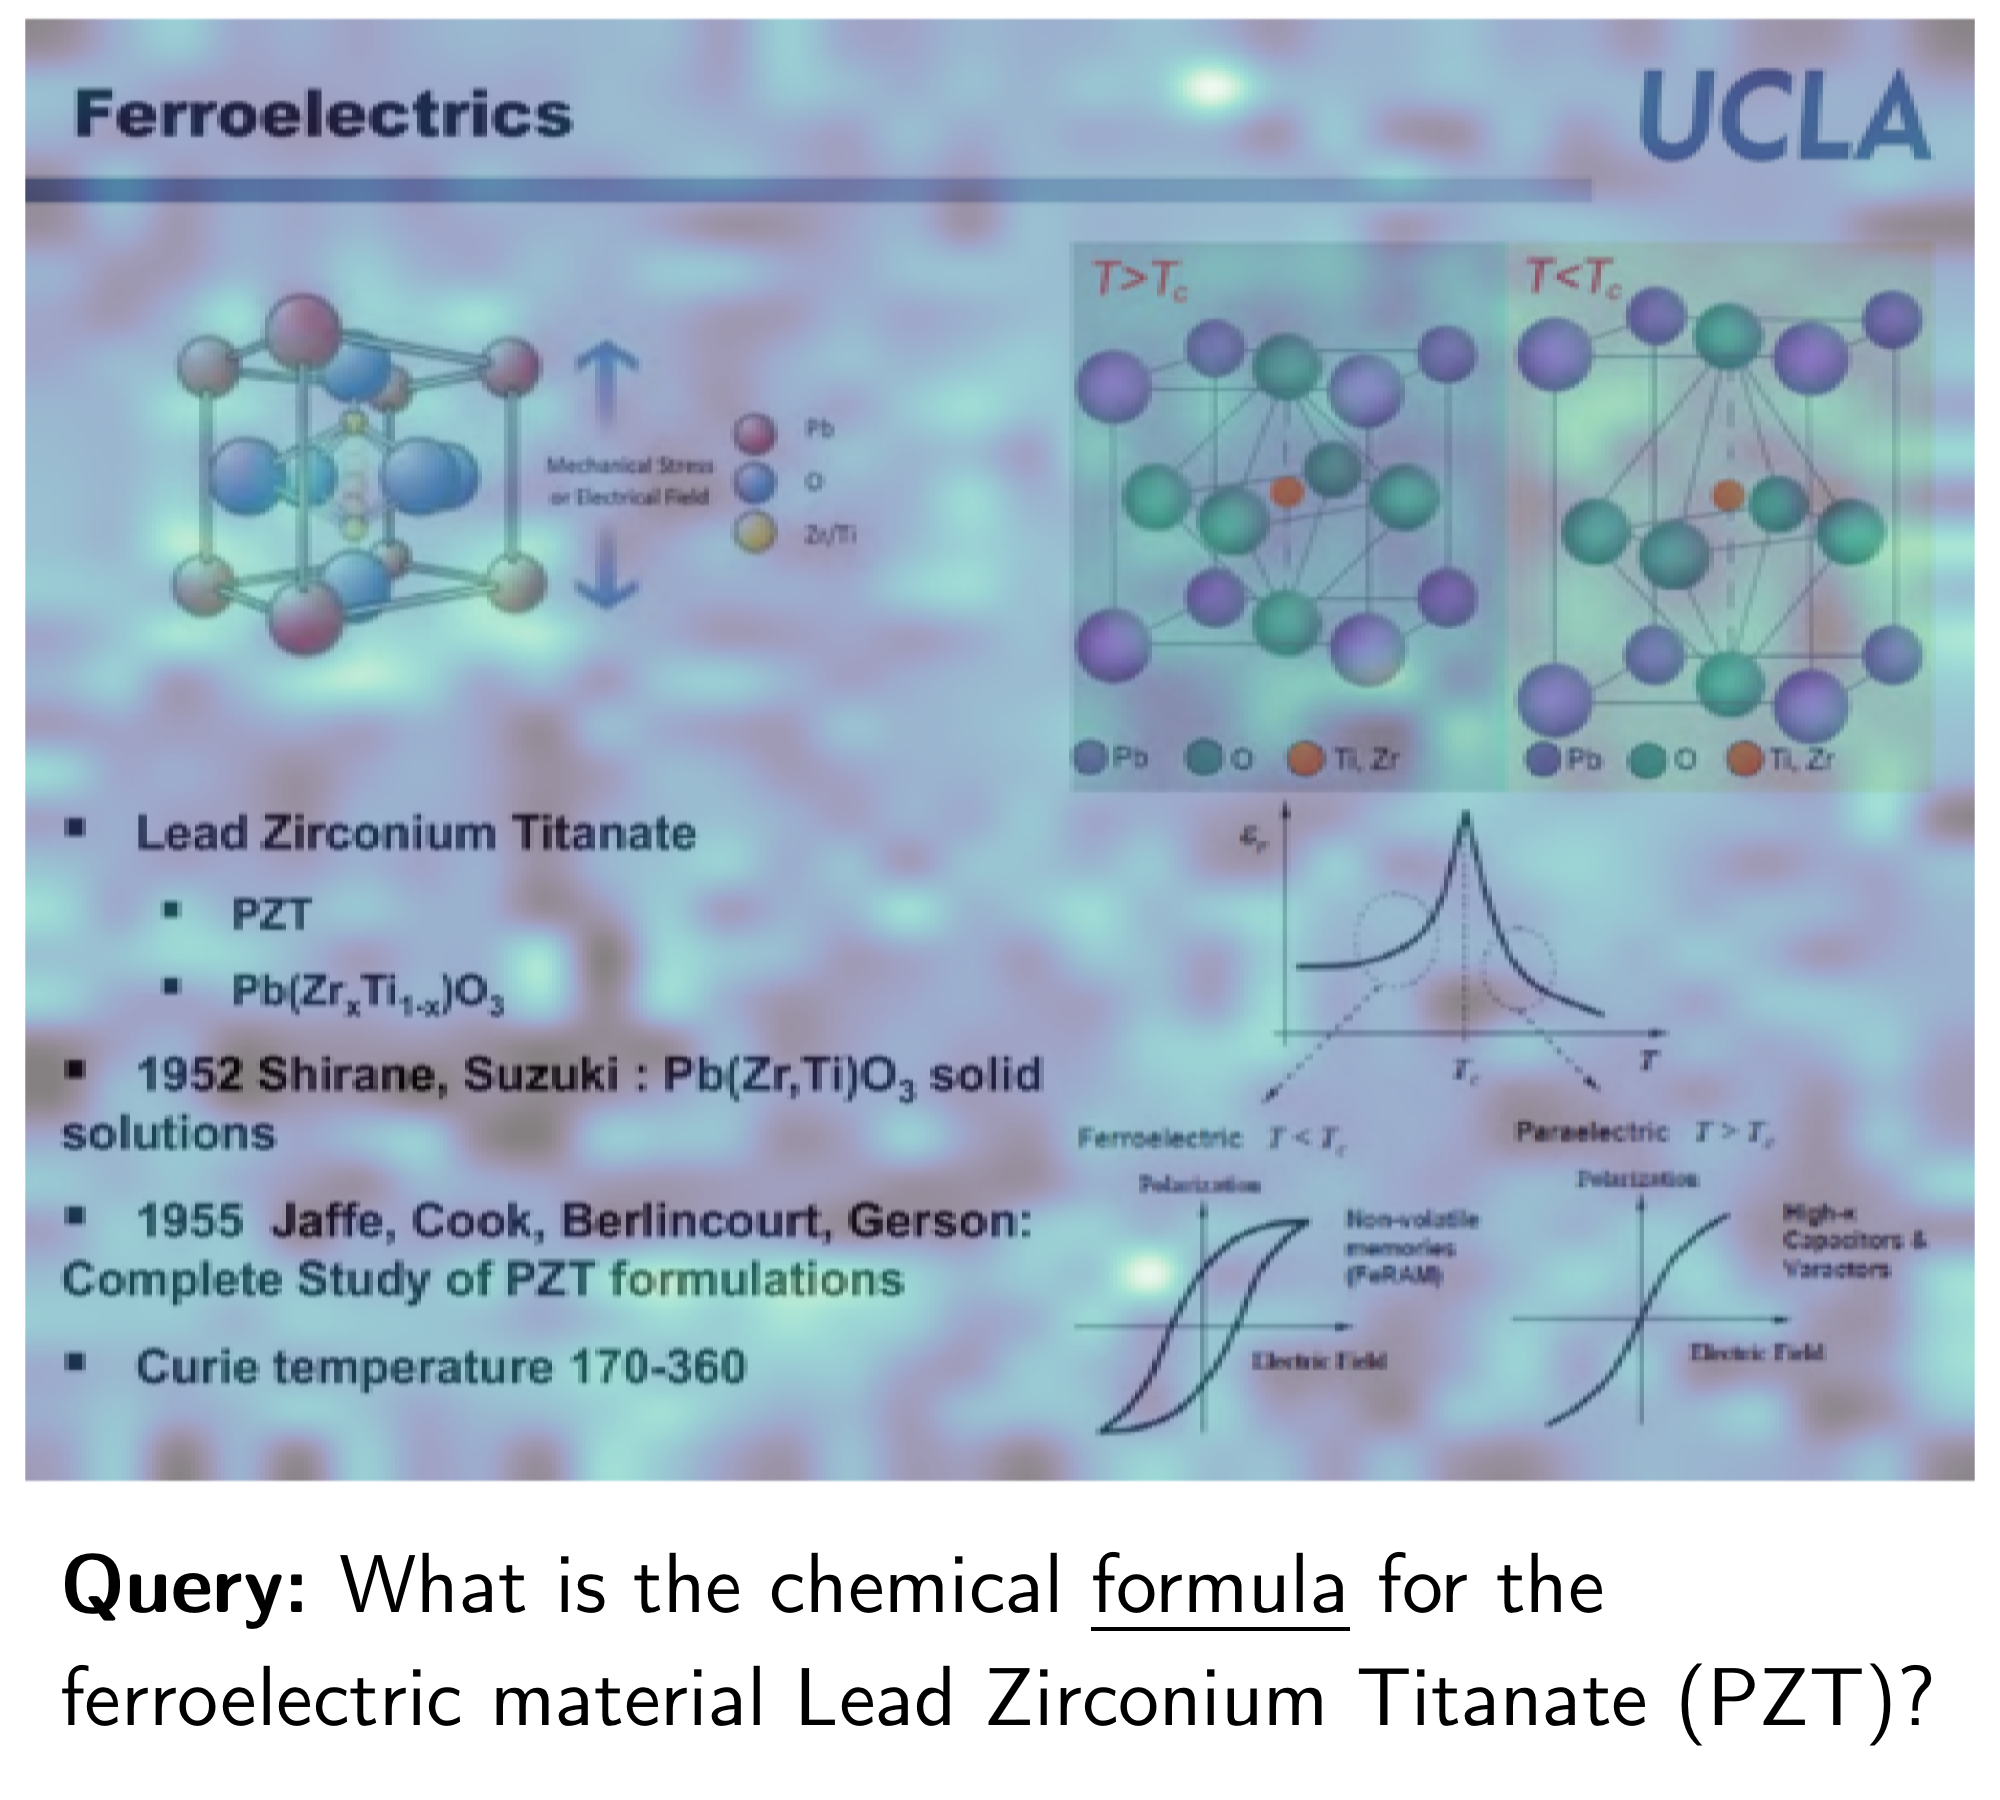
\includegraphics[width=0.95\linewidth]{images/colpali_images/similarity_maps/similarity_map_ferroelectrics.png} 
% \caption{Similarity of the image patches w.r.t. the underlined token in the user query. This example is from the \textit{Healthcare Industry} test set.}
% \label{fig:similarity_map_ferroelectrics}
% \end{figure}

% It is also interesting to highlight that both similarity maps showcase a few white patches with high similarity scores. This behavior might first seem surprising as the white patches should not carry a meaningful signal from the original images. We believe the vectors associated with these patches share a similar role with the ViT registers \sidecite{darcet_vision_2023}, i.e.\ these patches were repurposed for internal computations and stored the global information from the whole image.






\newpage
\onecolumn
\section{Additional results}


\subsection{Other Metrics}
\label{subection:additional_results}

% We share results for the Recall@1 metric which paints a similar picture in \autoref{table:results_appendix}.

\begin{table*}[ht]
    \centering
    
    \resizebox{\textwidth}{!}{%
    \begin{tabular}{ll@{\hskip 0.5em}l@{\hskip 0.5em}l@{\hskip 0.5em}l@{\hskip 0.5em}l@{\hskip 0.5em}l@{\hskip 0.5em}l@{\hskip 0.5em}l@{\hskip 0.5em}l@{\hskip 0.5em}l|@{\hskip 0.5em}l}

    \toprule
     & \textbf{ArxivQ} & \textbf{DocQ} & \textbf{InfoQ} & \textbf{TabF} & \textbf{TATQ} & \textbf{Shift} & \textbf{AI} & \textbf{Energy} & \textbf{Gov.} & \textbf{Health.} & \textbf{Avg.}\\
    
    
     % Captioning$_{\tiny \texttt{e5-large}}$ & 30.9\textcolor{red!75!black}{\tiny $\downarrow$-4.2} & 24.0\textcolor{red!75!black}{\tiny $\downarrow$-5.8} & 62.3\textcolor{green!75!black}{\tiny $\uparrow$0.8} & 54.3\textcolor{green!75!black}{\tiny $\uparrow$29.3} & 37.6\textcolor{red!75!black}{\tiny $\downarrow$-11.3} & 44.0\textcolor{red!75!black}{\tiny $\downarrow$-3.0} & 76.0\textcolor{red!75!black}{\tiny $\downarrow$-3.0} & 71.0\textcolor{red!75!black}{\tiny $\downarrow$-5.0} & 70.0\textcolor{red!75!black}{\tiny $\downarrow$-5.0} & 72.0\textcolor{red!75!black}{\tiny $\downarrow$-9.0} \\
    
    %%%%%
    \midrule
    \multicolumn{0}{l}{\textbf{\texttt{Unstructured} \tiny text-only}}\\% \textbf{Native \tiny(text)} &&&&&&&&&&\\
    BM25 & - & 26.6 & - & - & 34.6 & 45.0 & 86.0 & 70.0 & 68.0 & 74.0 & -  \\
    BGE-M3 & - & 22.8\textcolor{red!75!black}{\tiny $\downarrow$3.8} & - & - & 26.1\textcolor{red!75!black}{\tiny $\downarrow$8.5} & 51.0\textcolor{green!75!black}{\tiny $\uparrow$6.0} & 81.0\textcolor{red!75!black}{\tiny $\downarrow$5.0} & 72.0\textcolor{green!75!black}{\tiny $\uparrow$2.0} & 67.0\textcolor{red!75!black}{\tiny $\downarrow$1.0} & 77.0\textcolor{green!75!black}{\tiny $\uparrow$3.0} & -  \\
    \\
    \multicolumn{0}{l}{\textbf{\texttt{Unstructured \tiny+ OCR}}}\\
    BM25 & 26.7 & 28.9 & 54.0 & 30.4 & 50.0 & 52.0 & 86.0 & 77.0 & 74.0 & 80.0 & 55.9\\
    BGE-M3 & 
    28.1\textcolor{green!75!black}{\tiny $\uparrow$1.4} & 
    22.9\textcolor{red!75!black}{\tiny $\downarrow$6.0} & 53.8\textcolor{red!75!black}{\tiny $\downarrow$0.2} & 
    55.7\textcolor{green!75!black}{\tiny $\uparrow$25.3} & 
    38.6\textcolor{red!75!black}{\tiny $\downarrow$11.4} & 
    \textbf{56.0}\textcolor{green!75!black}{\tiny $\uparrow$4.0} & 82.0\textcolor{red!75!black}{\tiny $\downarrow$4.0} & 79.0\textcolor{green!75!black}{\tiny $\uparrow$2.0} & 
    76.0\textcolor{green!75!black}{\tiny $\uparrow$2.0} & 
    83.0\textcolor{green!75!black}{\tiny $\uparrow$3.0} & 
    57.5\textcolor{green!75!black}{\tiny $\uparrow$1.6}\\
    \\
    \multicolumn{0}{l}{\textbf{\texttt{Unstructured} \tiny+ Captioning}}\\
    BM25 & 35.5 & 30.2 & 61.5 & 24.3 & 49.0 & 47.0 & 79.0 & 76.0 & 75.0 & 81.0 & 55.9\\
    
    BGE-M3 & 
    29.3\textcolor{red!75!black}{\tiny $\downarrow$6.2} & 
    26.0\textcolor{red!75!black}{\tiny $\downarrow$4.2} & 
    62.1 \textcolor{green!75!black}{\tiny $\uparrow$0.6}& 
    58.6\textcolor{green!75!black}{\tiny $\uparrow$34.3} & 
    30.6\textcolor{red!75!black}{\tiny $\downarrow$18.4} & 
    55.0\textcolor{green!75!black}{\tiny $\uparrow$8.0} & 80.0\textcolor{green!75!black}{\tiny $\uparrow$1.0} & 
    78.0\textcolor{green!75!black}{\tiny $\uparrow$2.0} & 
    69.0\textcolor{red!75!black}{\tiny $\downarrow$6.0} & 
    83.0\textcolor{green!75!black}{\tiny $\uparrow$2.0} & 
    57.2\textcolor{green!75!black}{\tiny $\uparrow$1.3} \\
    \midrule

    % \textbf{Multimodal emb.} &\\
    \multicolumn{0}{l}{\textbf{Contrastive VLMs}}\\
    Jina-CLIP & 19.4 & 7.3 & 26.7 & 12.5 & 1.6 & 2.0 & 11.0 & 13.0 & 
    15.0 & 17.0 & 12.6\\
    Nomic-vision & 10.4 & 6.7 & 22.1 & 9.6 & 1.6 & 0.0 & 9.0 & 9.0 & 7.0 & 13.0 & 8.8\\
    SigLIP \tiny(Vanilla)& 34.2 & 21.3 & 51.8 & 46.1 & 17.9 & 13.0 & 50.0 & 51.0 & 47.0 & 65.0 & 39.7 \\
    %%%%%
    
    \midrule
    \multicolumn{0}{l}{\textbf{Ours}}\\
    SigLIP \tiny(Vanilla)& 34.2 & 21.3 & 51.8 & 46.1 & 17.9 & 13.0 & 50.0 & 51.0 & 47.0 & 65.0 & 39.7 \\
    BiSigLIP \tiny (+fine-tuning) & 49.2\textcolor{green!75!black}{\tiny $\uparrow$15.0} & 23.8\textcolor{green!75!black}{\tiny $\uparrow$2.5} & 59.0\textcolor{green!75!black}{\tiny $\uparrow$7.2} & 52.1\textcolor{green!75!black}{\tiny $\uparrow$6.0} & 20.7\textcolor{green!75!black}{\tiny $\uparrow$2.8} & 16.0\textcolor{green!75!black}{\tiny $\uparrow$3.0} & 62.0\textcolor{green!75!black}{\tiny $\uparrow$12.0} & 61.0\textcolor{green!75!black}{\tiny $\uparrow$10.0} & 55.0\textcolor{green!75!black}{\tiny $\uparrow$8.0} & 72.0\textcolor{green!75!black}{\tiny $\uparrow$7.0} & 47.1\textcolor{green!75!black}{\tiny $\uparrow$7.4}\\
    BiPali \tiny (+LLM) & 46.4\textcolor{red!75!black}{\tiny $\downarrow$-2.8} & 20.0\textcolor{red!75!black}{\tiny $\downarrow$-3.8} & 54.6\textcolor{red!75!black}{\tiny $\downarrow$-4.4} & 63.2\textcolor{green!75!black}{\tiny $\uparrow$11.1} & 20.4\textcolor{red!75!black}{\tiny $\downarrow$-0.4} & 34.0\textcolor{green!75!black}{\tiny $\uparrow$18.0} & 59.0\textcolor{red!75!black}{\tiny $\downarrow$-3.0} & 45.0\textcolor{red!75!black}{\tiny $\downarrow$-16.0} & 57.0\textcolor{green!75!black}{\tiny $\uparrow$2.0} & 56.0\textcolor{red!75!black}{\tiny $\downarrow$-16.0} & 45.6\textcolor{red!75!black}{\tiny $\downarrow$-1.5}\\
    \textit{ColPali} \tiny (+Late Inter.) & \textbf{72.4}\textcolor{green!75!black}{\tiny $\uparrow$26.0} & \textbf{45.6}\textcolor{green!75!black}{\tiny $\uparrow$25.6} & \textbf{74.6}\textcolor{green!75!black}{\tiny $\uparrow$20.0} & \textbf{75.4}\textcolor{green!75!black}{\tiny $\uparrow$12.1} & \textbf{53.1}\textcolor{green!75!black}{\tiny $\uparrow$32.7} & 55.0\textcolor{green!75!black}{\tiny $\uparrow$21.0} & \textbf{93.0}\textcolor{green!75!black}{\tiny $\uparrow$34.0} & \textbf{85.0}\textcolor{green!75!black}{\tiny $\uparrow$40.0} & \textbf{85.0}\textcolor{green!75!black}{\tiny $\uparrow$28.0} & \textbf{88.0}\textcolor{green!75!black}{\tiny $\uparrow$32.0} & \textbf{72.7}\textcolor{green!75!black}{\tiny $\uparrow$27.1}\\
    \bottomrule
    \end{tabular}
    }
    

    \caption[\textsc{ViDoRe} Recall@1 evaluation]{\textbf{Comprehensive evaluation of baseline models and our proposed method on \textsc{ViDoRe}.} Results are presented using Recall@1 metrics. Text-only metrics are not computed for benchmarks with only visual elements.}
    \label{table:results_appendix}
\end{table*}


\subsection{Model Variants}
\label{subection:model_variants}


% \begin{figure}[ht]
%     \centering
%     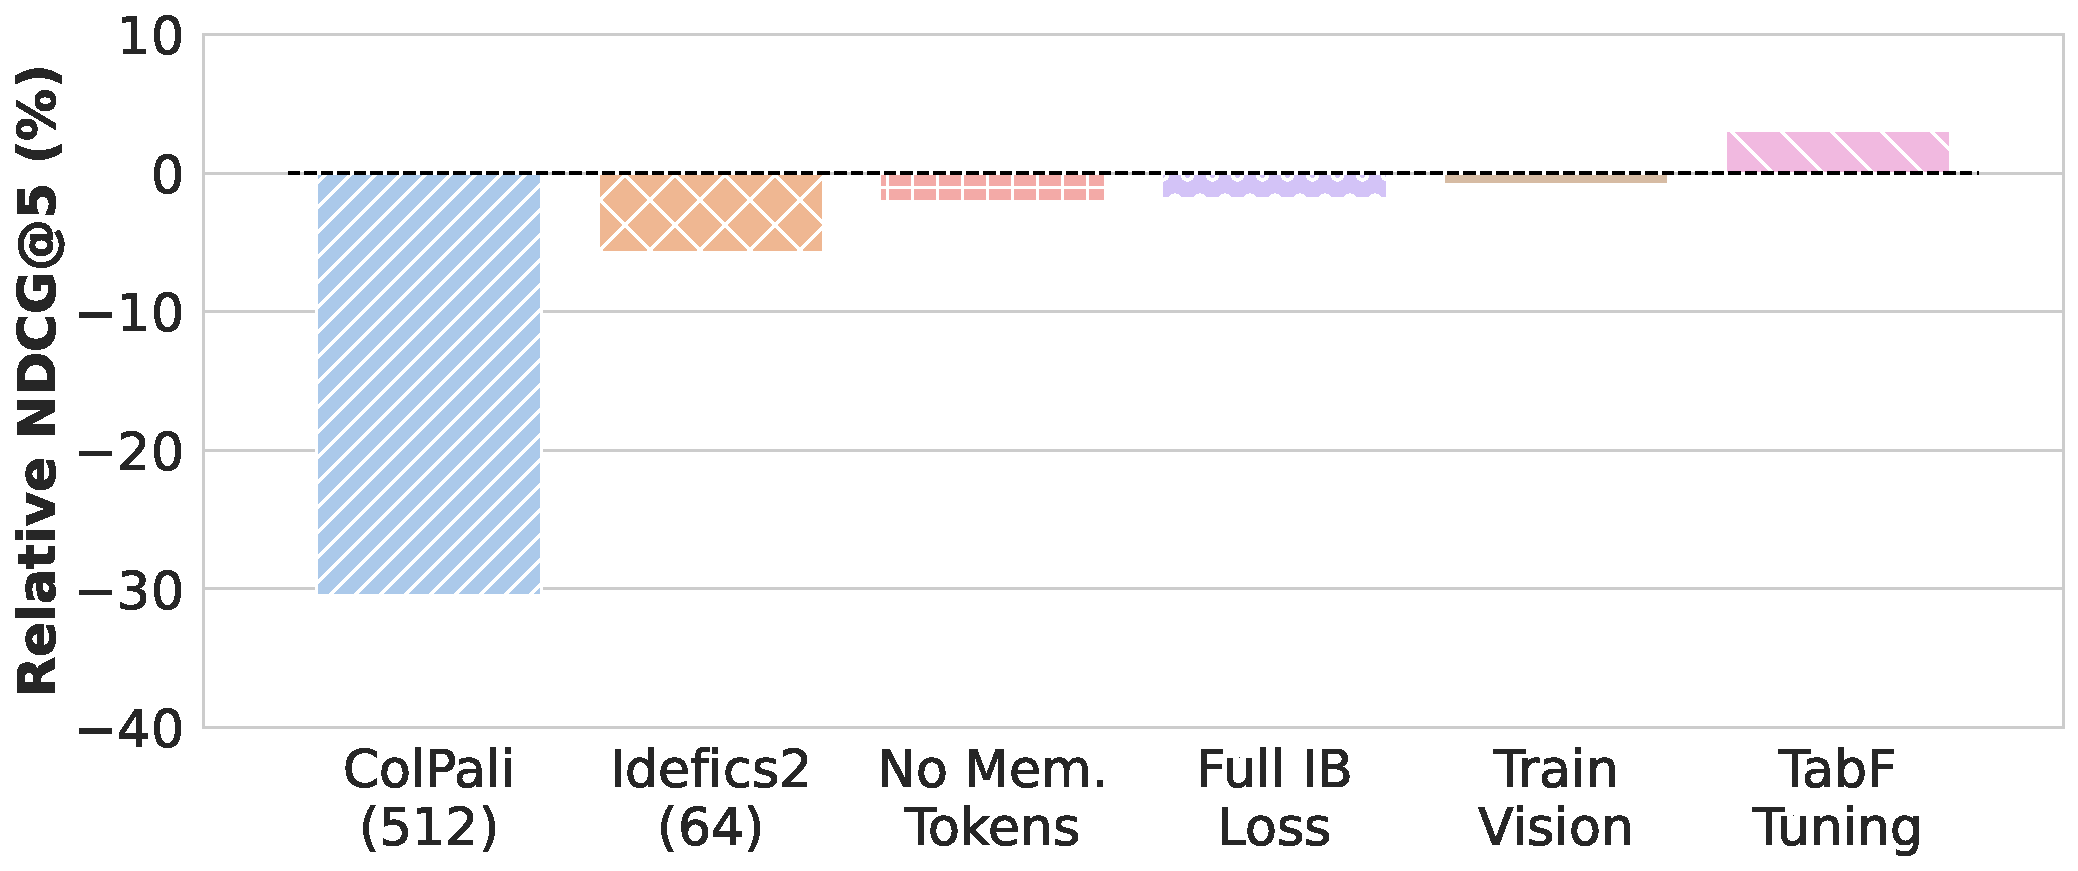
\includegraphics[width = 0.8\linewidth]{images/colpali_images/ablations.pdf}
%     \caption{Relative nDCG@5 performance gain w.r.t. the default \textit{ColPali} (1024 patches). \textit{TabFQuAD fine-tuning} measures the performance difference on the TabFQuAD task after the introduction of targeted data in the training set. All other results refer to performance deltas averaged on all \textit{ViDoRe} tasks.}
%     \label{fig:ablations}
% \end{figure}


\begin{table*}[ht]
    \centering
    
    \resizebox{\textwidth}{!}{%
    \begin{tabular}{ll@{\hskip 0.5em}l@{\hskip 0.5em}l@{\hskip 0.5em}l@{\hskip 0.5em}l@{\hskip 0.5em}l@{\hskip 0.5em}l@{\hskip 0.5em}l@{\hskip 0.5em}l@{\hskip 0.5em}l|@{\hskip 0.5em}l}

    \toprule
     & \textbf{ArxivQ} & \textbf{DocQ} & \textbf{InfoQ} & \textbf{TabF} & \textbf{TATQ} & \textbf{Shift} & \textbf{AI} & \textbf{Energy} & \textbf{Gov.} & \textbf{Health.} & \textbf{Avg.}\\
    \midrule
        ColSigLIP (PaliGemma) & 3.1 & 3.0 & 5.1 & 6.2 & 2.5 & 1.0 & 3.4 & 3.4 & 2.3 & 2.2 & 3.2 \\
        BiSigLIP (PaliGemma) & 18.5 & 14.6 & 33.4 & 39.5 & 16.1 & 5.2 & 27.6 & 32.6 & 36.6 & 35.7 & 26.0 \\
        ColSigLIP (Original) & 2.6 & 2.2 & 2.3 & 5.7 & 1.8 & 1.0 & 2.6 & 4.1 & 1.4 & 1.5 & 2.5 \\
    \midrule
        ColPali (No Q.A. Tokens) & 80.4 & 53.2 & 82.4 & 77.4 & 65.7 & 63.4 & 97.0 & 89.9 & 93.6 & 92.4 & 79.6 \\
        ColPali (Docmatix) & 71.3 & 48.0 & 80.0 & 83.9 & 59.1 & 73.8 & 95.7 & 93.8 & 92.5 & 93.1 & 79.1 \\
        ColPali (224) & 71.0 & 37.4 & 62.3 & 65.7 & 28.6 & 20.4 & 65.7 & 66.8 & 73.9 & 73.0 & 56.5 \\
        ColPali (Vision Trained) & 78.8 & 53.9 & 81.3 & 81.7 & 64.4 & 70.6 & 95.3 & 91.7 & 93.5 & 94.7 & 80.6 \\
        ColPali (No Pairwise) & 79.0 & 53.0 & 82.1 & 85.3 & 63.2 & 66.2 & 94.9 & 88.9 & 92.7 & 92.1 & 79.7 \\
        ColPali (+TabFQuAD training) & 77.6 & 54.7 & 82.6 & 86.5 & 65.4 & 73.9 & 94.8 & 92.4 & \textbf{94.2} & 94.8 & 81.7 \\

        ColIdefics2  (64)      & 73.6 & 48.0 & 82.4 & 81.6 & 63.0 & 57.2 & 95.5 & 86.9 & 86.6 & 91.2 & 76.6 \\
        ColQwen2  (768)         & \textbf{86.4} & \textbf{56.2} & \textbf{89.8} & \textbf{88.7} & \textbf{75.2} & \textbf{85.7} & \textbf{98.8} & \textbf{94.8} & 93.6 & \textbf{97.3} & \textbf{86.6} \\
    \midrule
        \textit{ColPali} (Reference: 448) & 79.1 & 54.4 & 81.8 & 83.9 & 65.8 & 73.2 & 96.2 & 91.0 & 92.7 & 94.4 & 81.3 \\
            \bottomrule
    \end{tabular}
    }
    

    \caption[\textsc{ViDoRe} ablations and negative results]{\textbf{Benchmark scores for the ``negative results" and various ablations on \textsc{ViDoRe}; \textit{ColPali} for reference.} Results are presented using nDCG@5 metrics. Text-only metrics are not computed for benchmarks with only visual elements.}
    \label{table:negative_results}
\end{table*}





\newpage
\section{More similarity maps}
\label{section:more_similarity_maps}
In \autoref{fig:similarity_map_kazakhstan}, \textit{ColPali} assigns a high similarity to all patches with the word \textit{``Kazakhstan"} when given the token \texttt{<\_Kazakhstan>}. Moreover, our model seems to exhibit world knowledge capabilities as the patch around the word \textit{"Kashagan"}—an offshore oil field in Kazakhstan—also shows a high similarity score.

\begin{figure}
\centering
    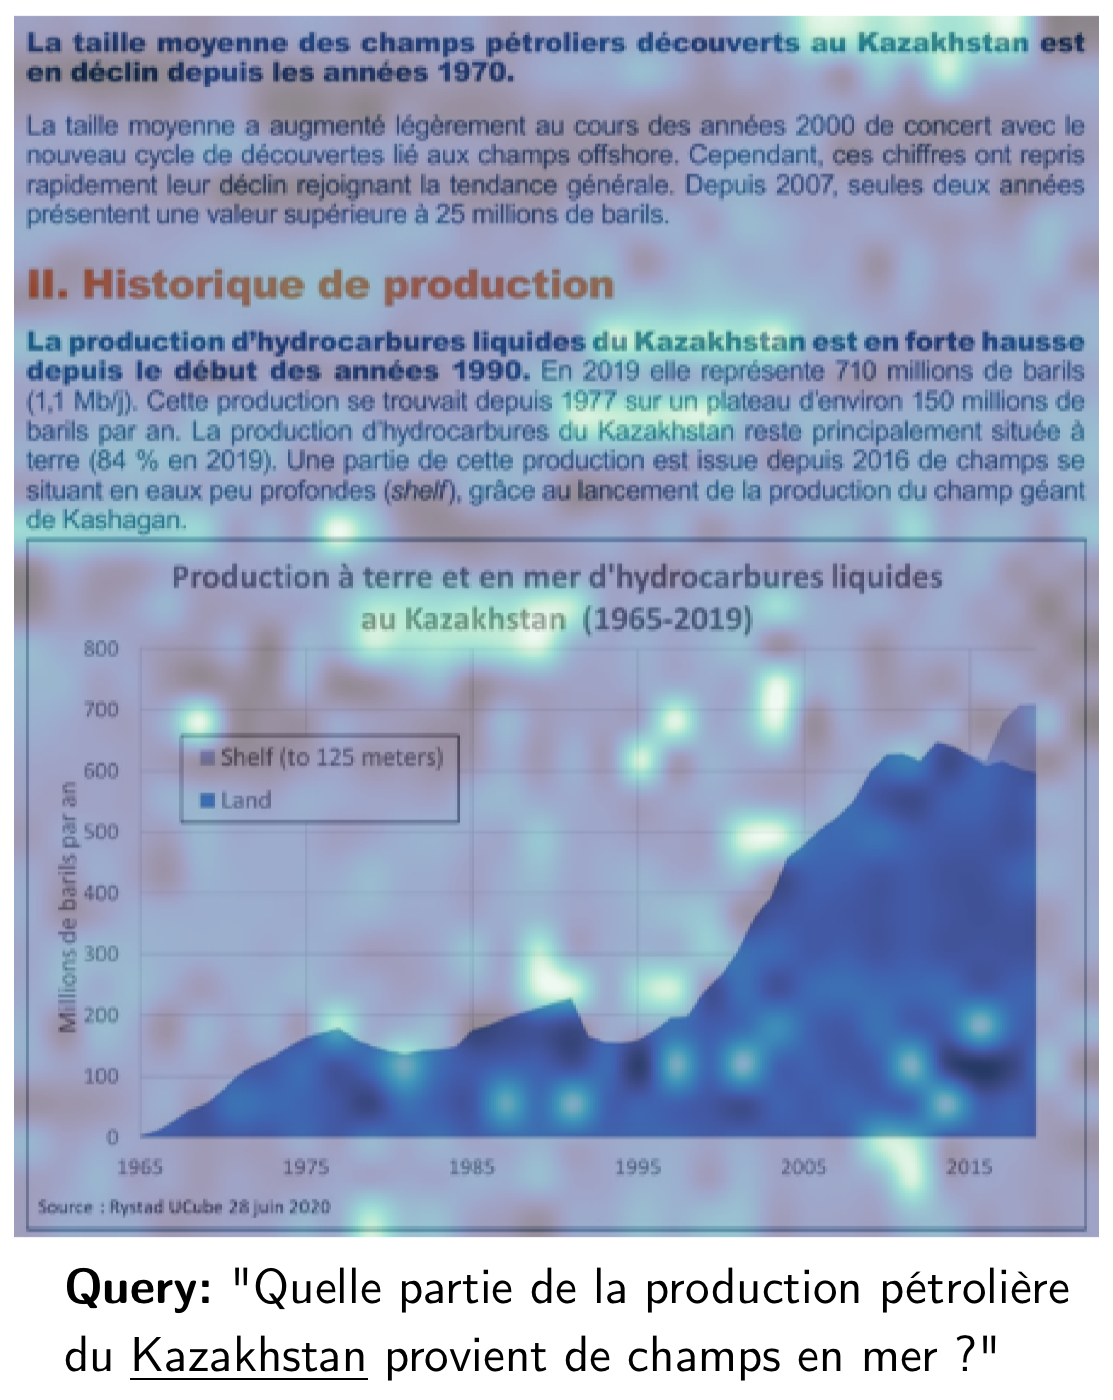
\includegraphics[width=0.5\linewidth]{images/colpali_images/similarity_maps/similarity_map_kazakhstan.png} 
    \caption[Similarity map example]{Similarity of the image patches w.r.t. the underlined token in the user query. This example is from the \textit{Shift} test set.}
\label{fig:similarity_map_kazakhstan}
\end{figure}

It is also interesting to highlight that both this similarity map and the one displayed in \autoref{fig:similarity-maps} showcase a few white patches with high similarity scores. This behavior might first seem surprising as the white patches should not carry a meaningful signal from the original images. We believe the vectors associated with these patches share a similar role with the ViT registers \sidecite{darcet_vision_2023}, i.e.\ these patches were repurposed for internal computations and stored the global information from the whole image.

\section{Model glossary}
\label{section:model_glossary}


\subsection*{SigLIP}
\label{subsection:glossary_siglip}

SigLIP (Sigmoid Loss for Language Image Pre-Training) builds upon CLIP (Contrastive Language-Image Pretraining)—a foundational model that aligns images and text by maximizing the similarity between correct image-text pairs while minimizing it for incorrect ones, leveraging a contrastive loss \sidecite{zhai_sigmoid_2023}. Unlike CLIP \sidecite{radford_learning_2021}, which applies the softmax function to the logits, SigLIP uses the sigmoid activation function. This innovation eliminates the need for a global view of all pairwise similarities between images and texts within a batch, enabling more flexible batch size scaling (up to 1M items per batch, with an effective optimal batch size of 32k). This approach allows SigLIP to achieve state-of-the-art performance in zero-shot image classification tasks.


\subsection*{PaliGemma}
\label{subsection:glossary_paligemma}

PaliGemma is a 3B-parameter vision-language model. It integrates the SigLIP vision encoder with a Gemma-2B language decoder, connected via a multimodal linear projection layer \sidecite{lucas_beyer_paligemma_2024}. The model processes images by segmenting them into a fixed number of Vision Transformer \sidecite{dosovitskiy_image_2020} tokens, which are prepended to an optional text prompt.

A distinguishing feature of PaliGemma is its operation as a Prefix-Language Model (Prefix-LM). This design ensures full attention between image tokens and the user-provided input (prefix) while generating outputs auto-regressively (suffix). This architecture allows image tokens to access the task-specific query during processing, facilitating more effective task-dependent reasoning.

PaliGemma was trained in four stages: unimodal pretraining with existing components, extended multimodal pretraining, short high-resolution pretraining, and task-specific fine-tuning.


\subsection*{ColBERT}
\label{subsection:glossary_colbert}

ColBERT (Contextualized Late Interaction over BERT) is a retrieval model designed to balance speed and effectiveness in information retrieval tasks \sidecite{khattab2020colbert}. Traditional retrieval models are typically categorized based on their type of interaction: either processing queries and documents independently for efficiency (bi-encoders) or jointly to capture rich contextual relationships (cross-encoders). ColBERT combines the advantages of both approaches through a novel late interaction mechanism.

Queries and documents are encoded separately using BERT, enabling offline pre-computation of document representations for scalability. Instead of pooling embeddings into a single vector, ColBERT retains token-level embeddings and employs a MaxSim operator to compute fine-grained similarity scores. For each query token, the model determines the maximum similarity with document tokens, summing these scores to compute relevance.

This architecture preserves the contextual richness of deep language models while significantly improving computational efficiency. By delaying the interaction step, ColBERT supports vector similarity indexing, facilitating end-to-end retrieval from large collections without prohibitive costs. Empirical evaluations on passage search datasets demonstrate that ColBERT achieves competitive effectiveness compared to existing BERT-based models \sidecite{devlin2019bert}, while executing queries orders of magnitude faster and with drastically reduced computational requirements.


\newpage
\section{Examples from the \textsc{ViDoRe} benchmark}
\label{subsection:docvisbenchmark_examples}

\vspace*{3\baselineskip}

\begin{center}
    \textbf{Energy} \\[1ex]
    \begin{figure}[h]
        \centering
        \begin{subfigure}[t]{0.30\textwidth}
            \caption*{\textbf{Query}: What types of accounts or products allow investors to defer paying taxes?}
            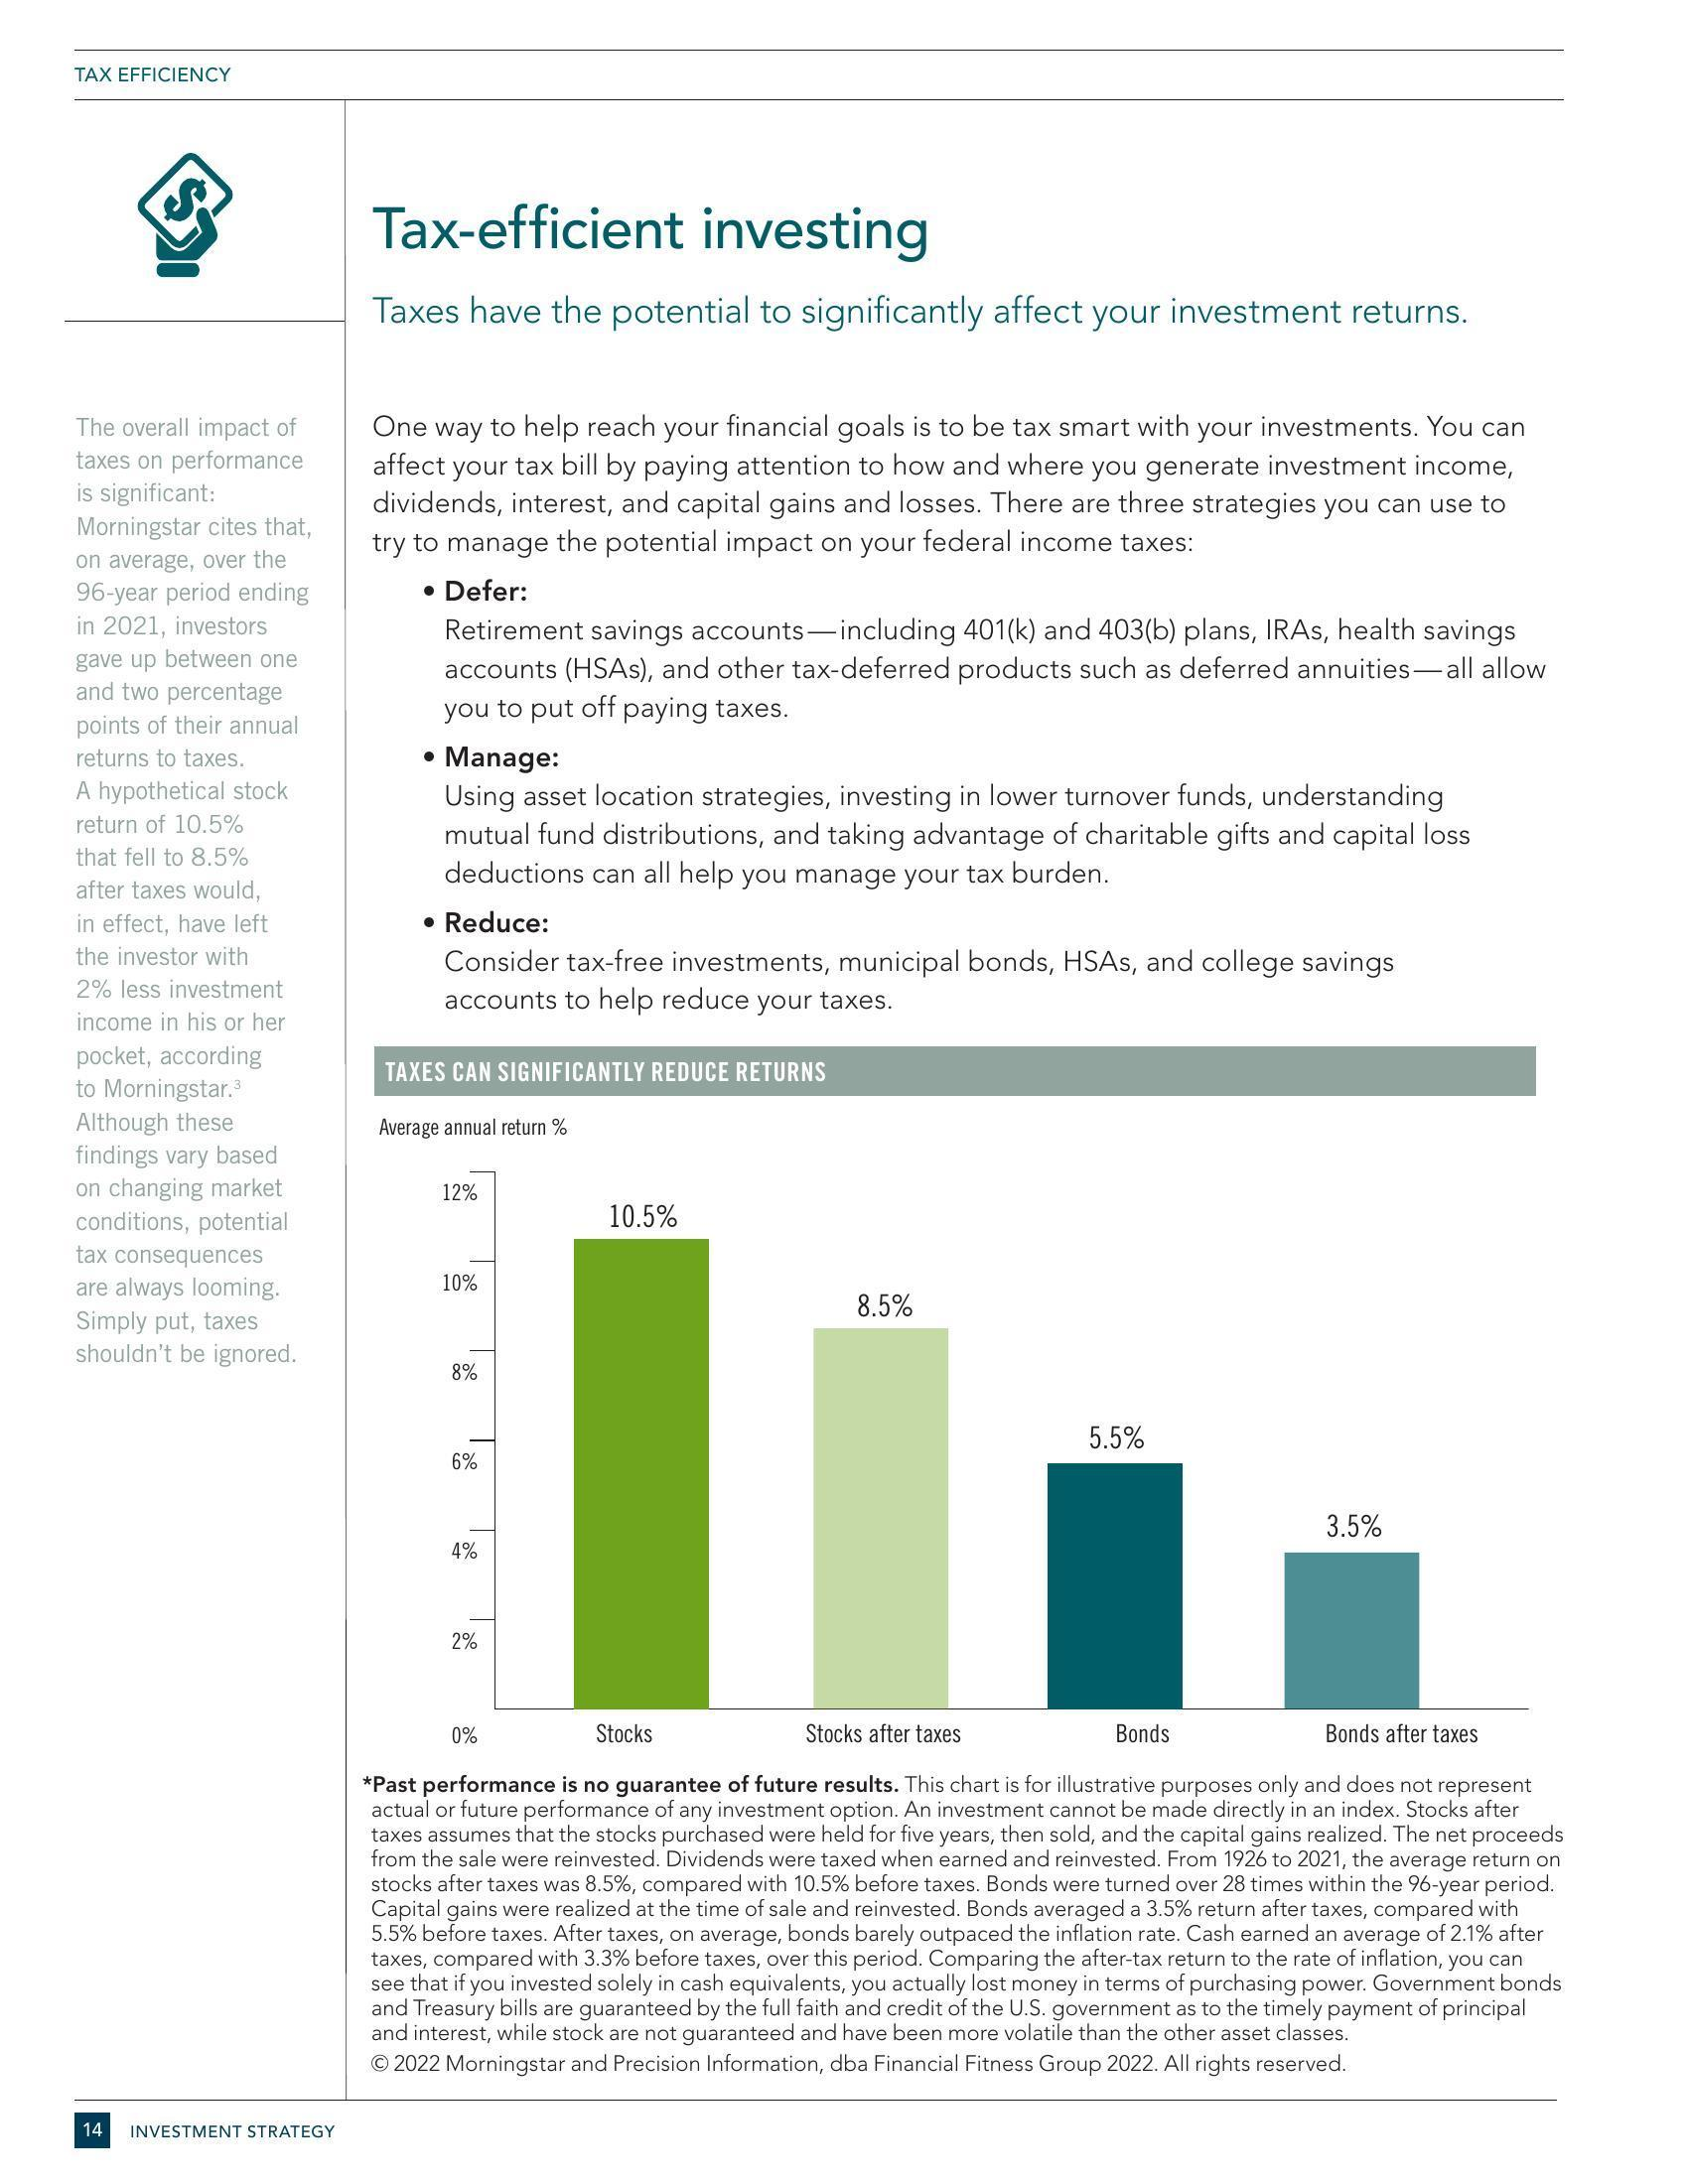
\includegraphics[width=\textwidth]{images/colpali_images/dataset_samples/energy_1.jpeg}
        \end{subfigure} \ 
        \begin{subfigure}[t]{0.30\textwidth}
            \caption*{\textbf{Query}: What is the estimated total savings for a PV system in Durham under the net metering (flat rate) billing option over the system's useful life of 25 years?}
            \includegraphics*[width=\textwidth]{images/colpali_images/dataset_samples/energy_2.jpeg}
        \end{subfigure}
        \begin{subfigure}[t]{0.30\textwidth}
            \caption*{\textbf{Query}: What is the projected peak electricity demand in California for the year 2030?}
            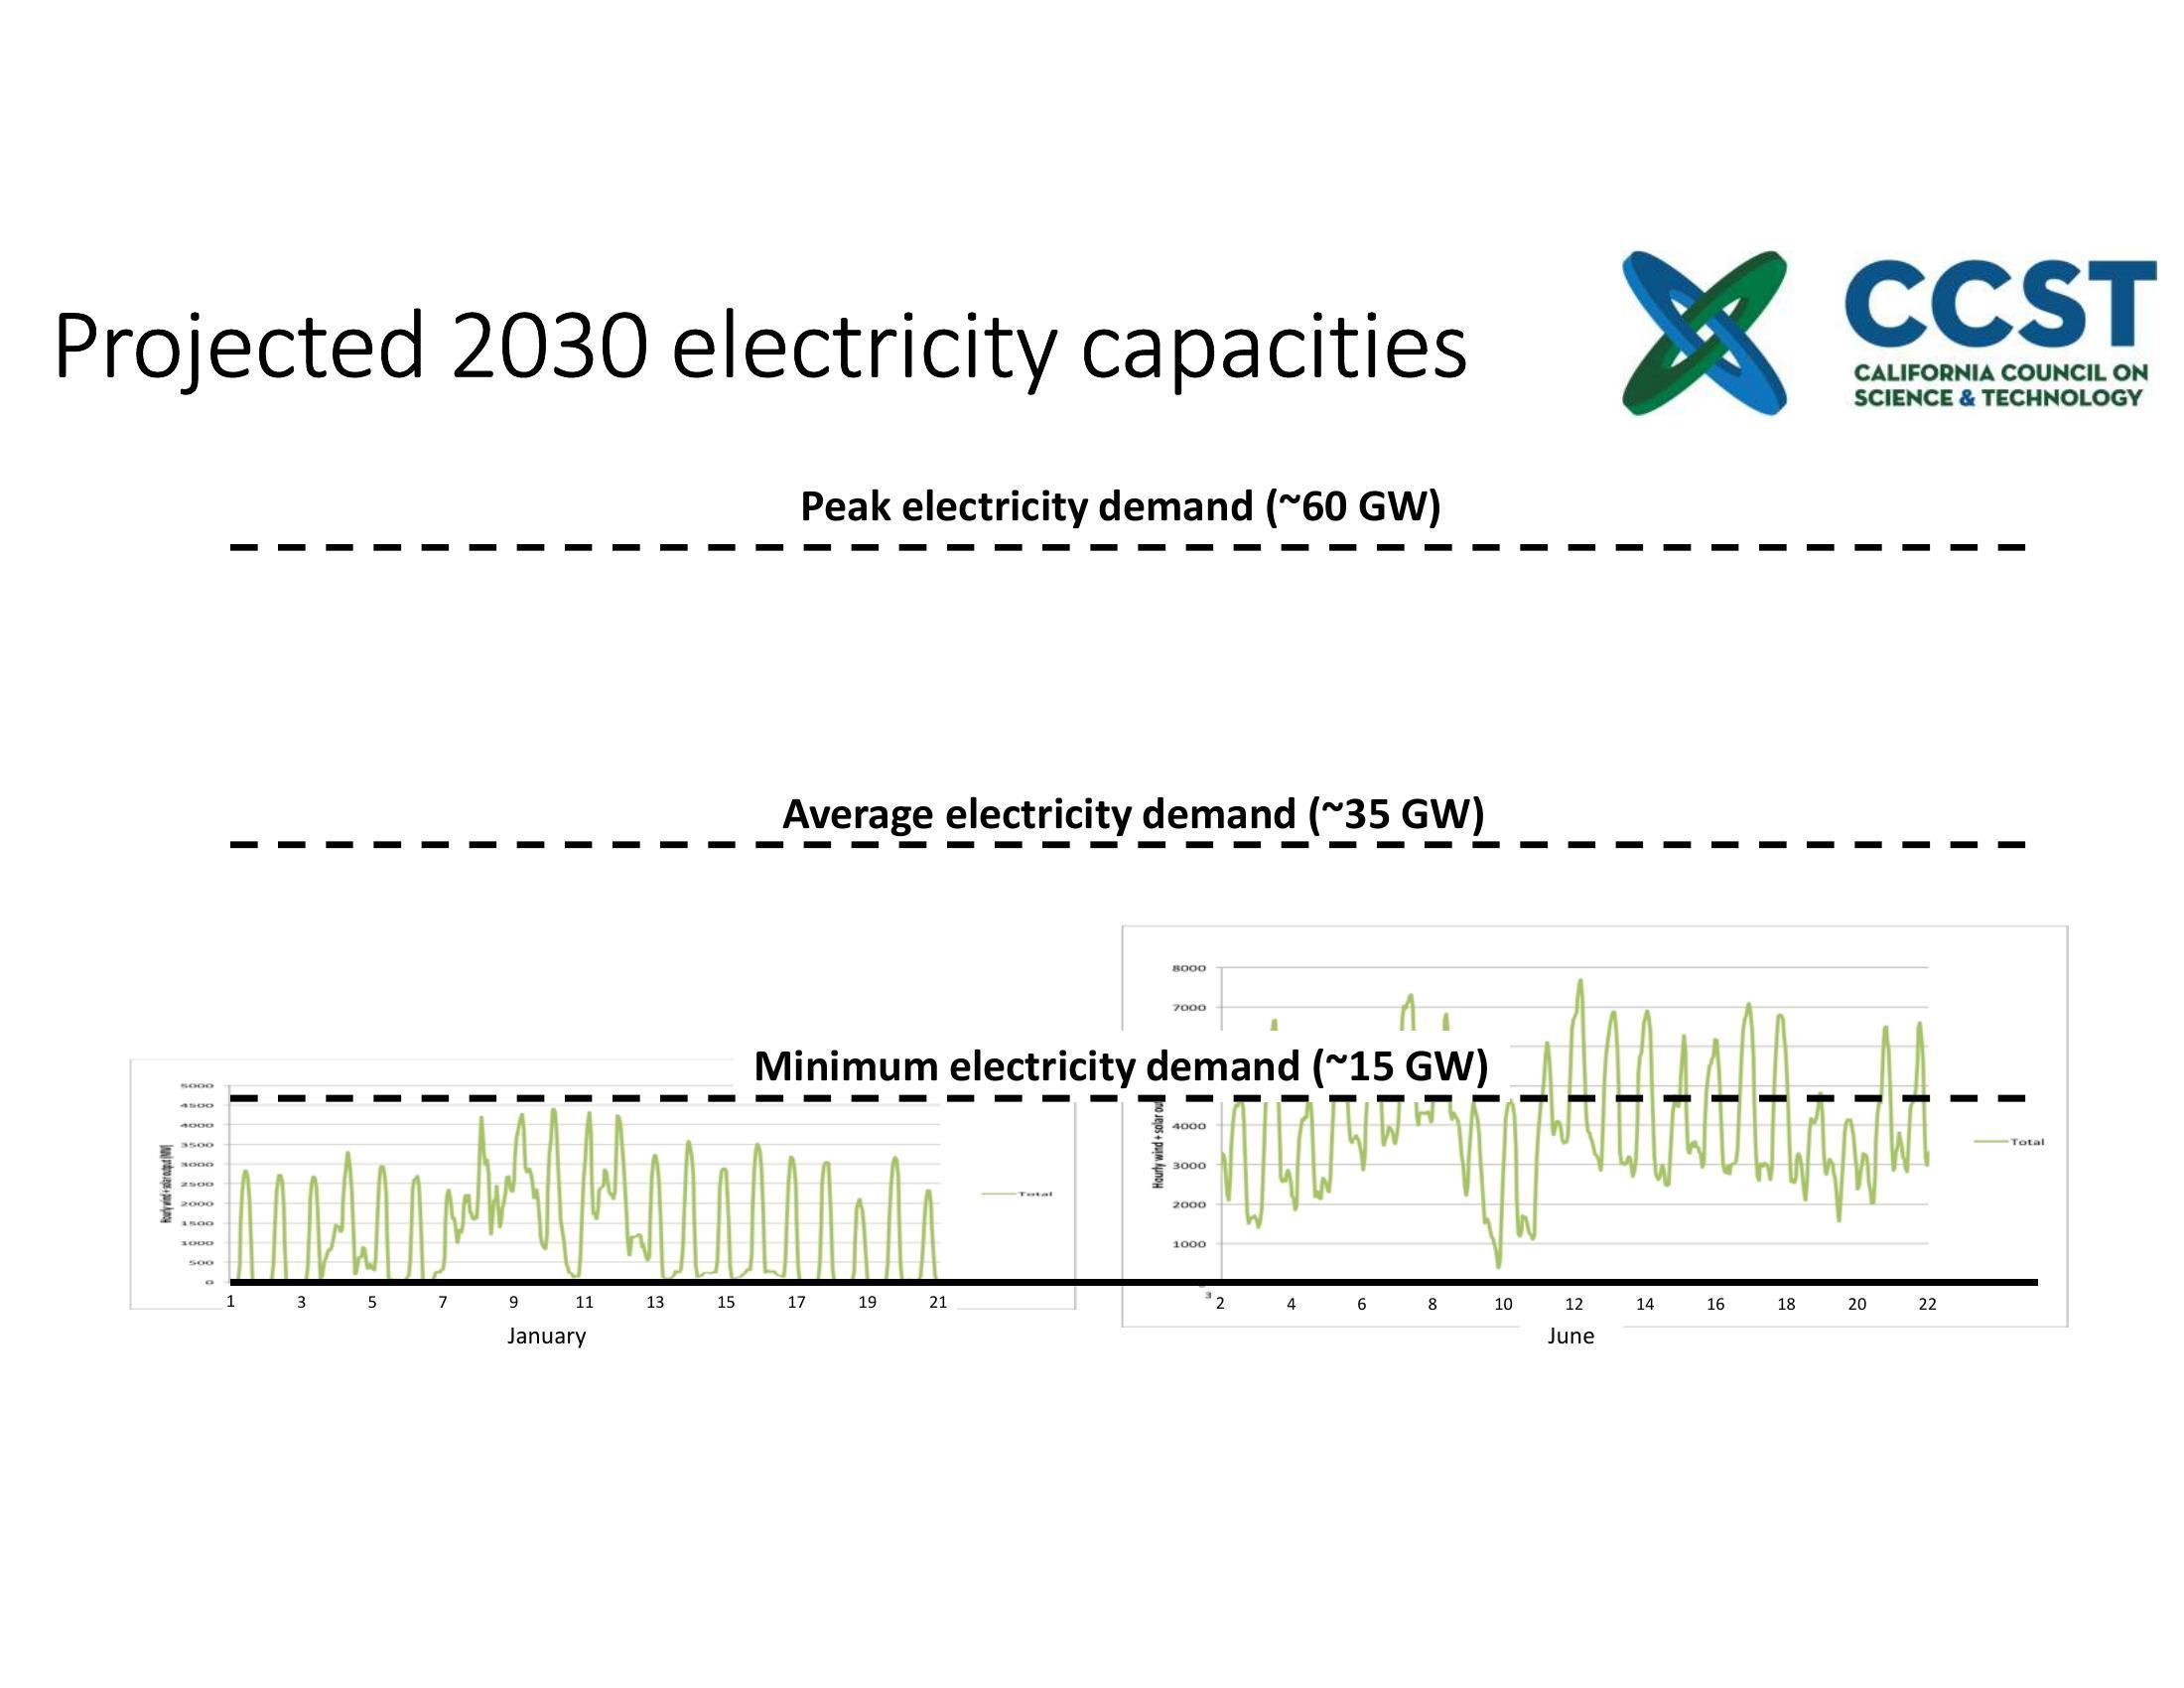
\includegraphics[width=\textwidth]{images/colpali_images/dataset_samples/energy_3.jpeg}
        \end{subfigure} \ 
    \end{figure}

    \vspace*{5\baselineskip}
    
    \textbf{Artificial Intelligence} \\[1ex]
    \begin{figure}[h]
        \centering
        \begin{subfigure}[t]{0.30\textwidth}
            \caption*{\textbf{Query}: What are some common outcome areas targeted by TAII for different age groups?}
            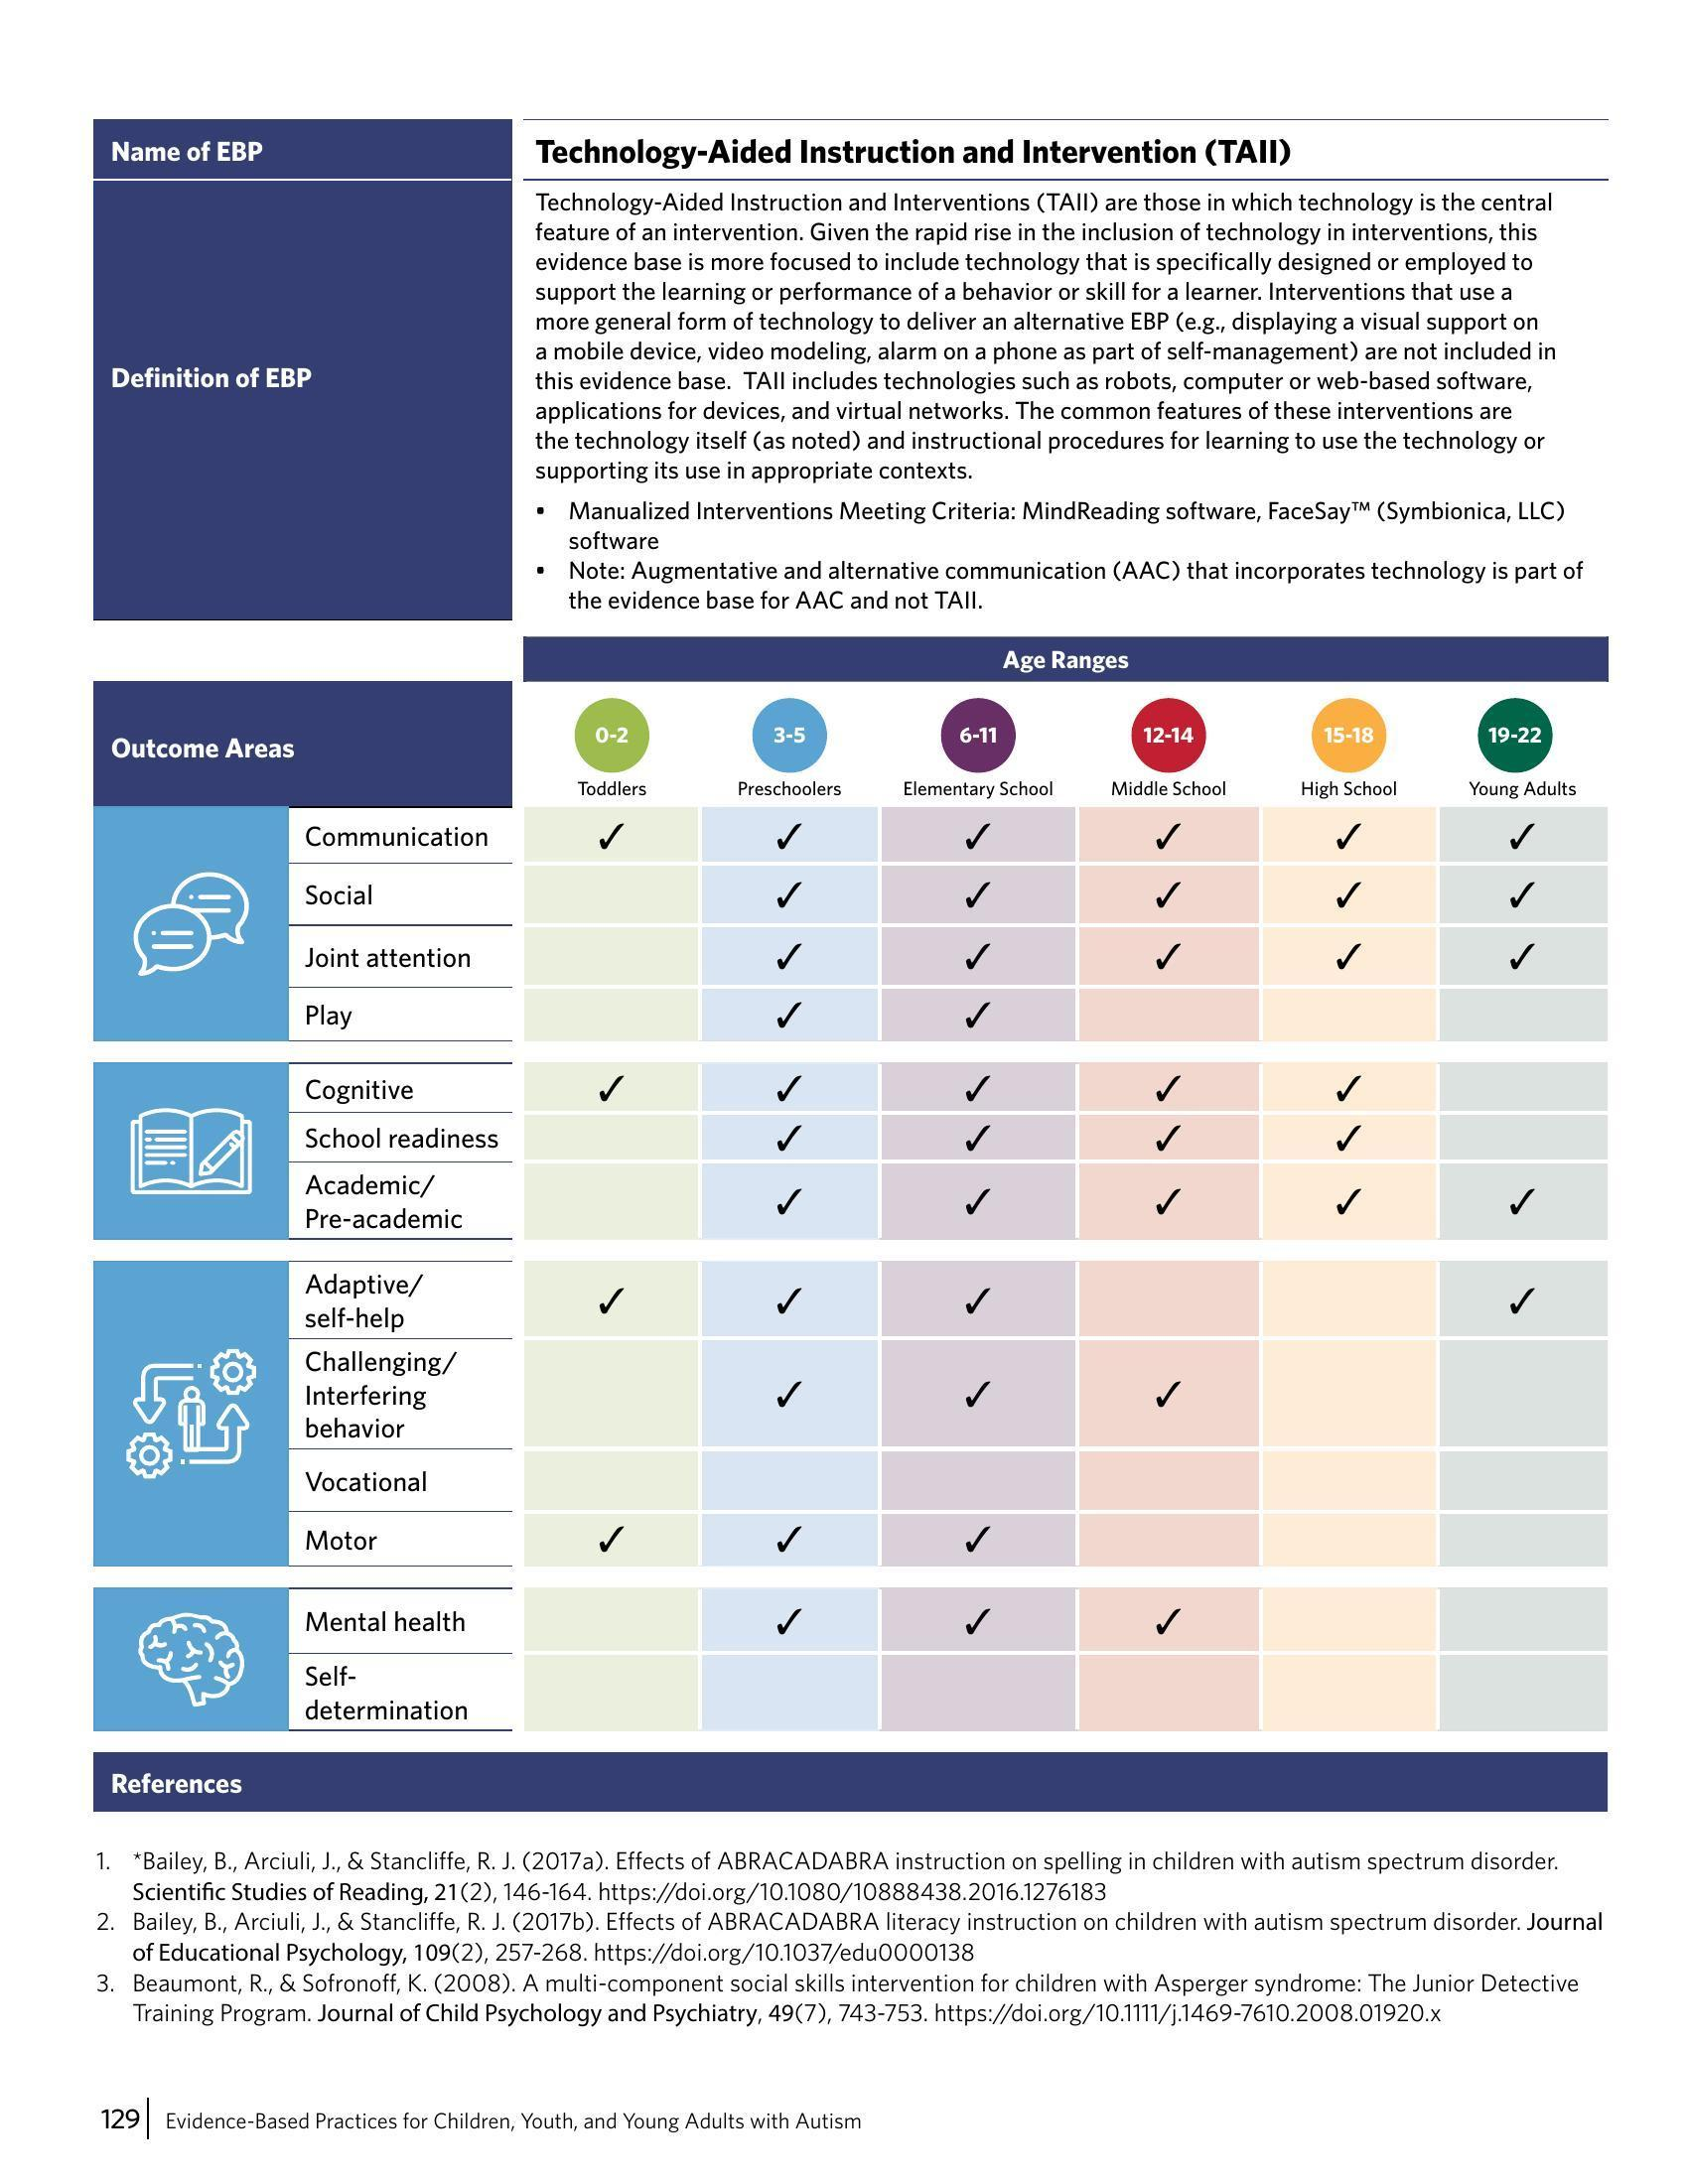
\includegraphics[width=\textwidth]{images/colpali_images/dataset_samples/ai_1.jpeg}
        \end{subfigure} \ 
        \begin{subfigure}[t]{0.30\textwidth}
            \caption*{\textbf{Query}: What did the robot monitor to determine when to activate or deactivate the blower motor and blinker?}
            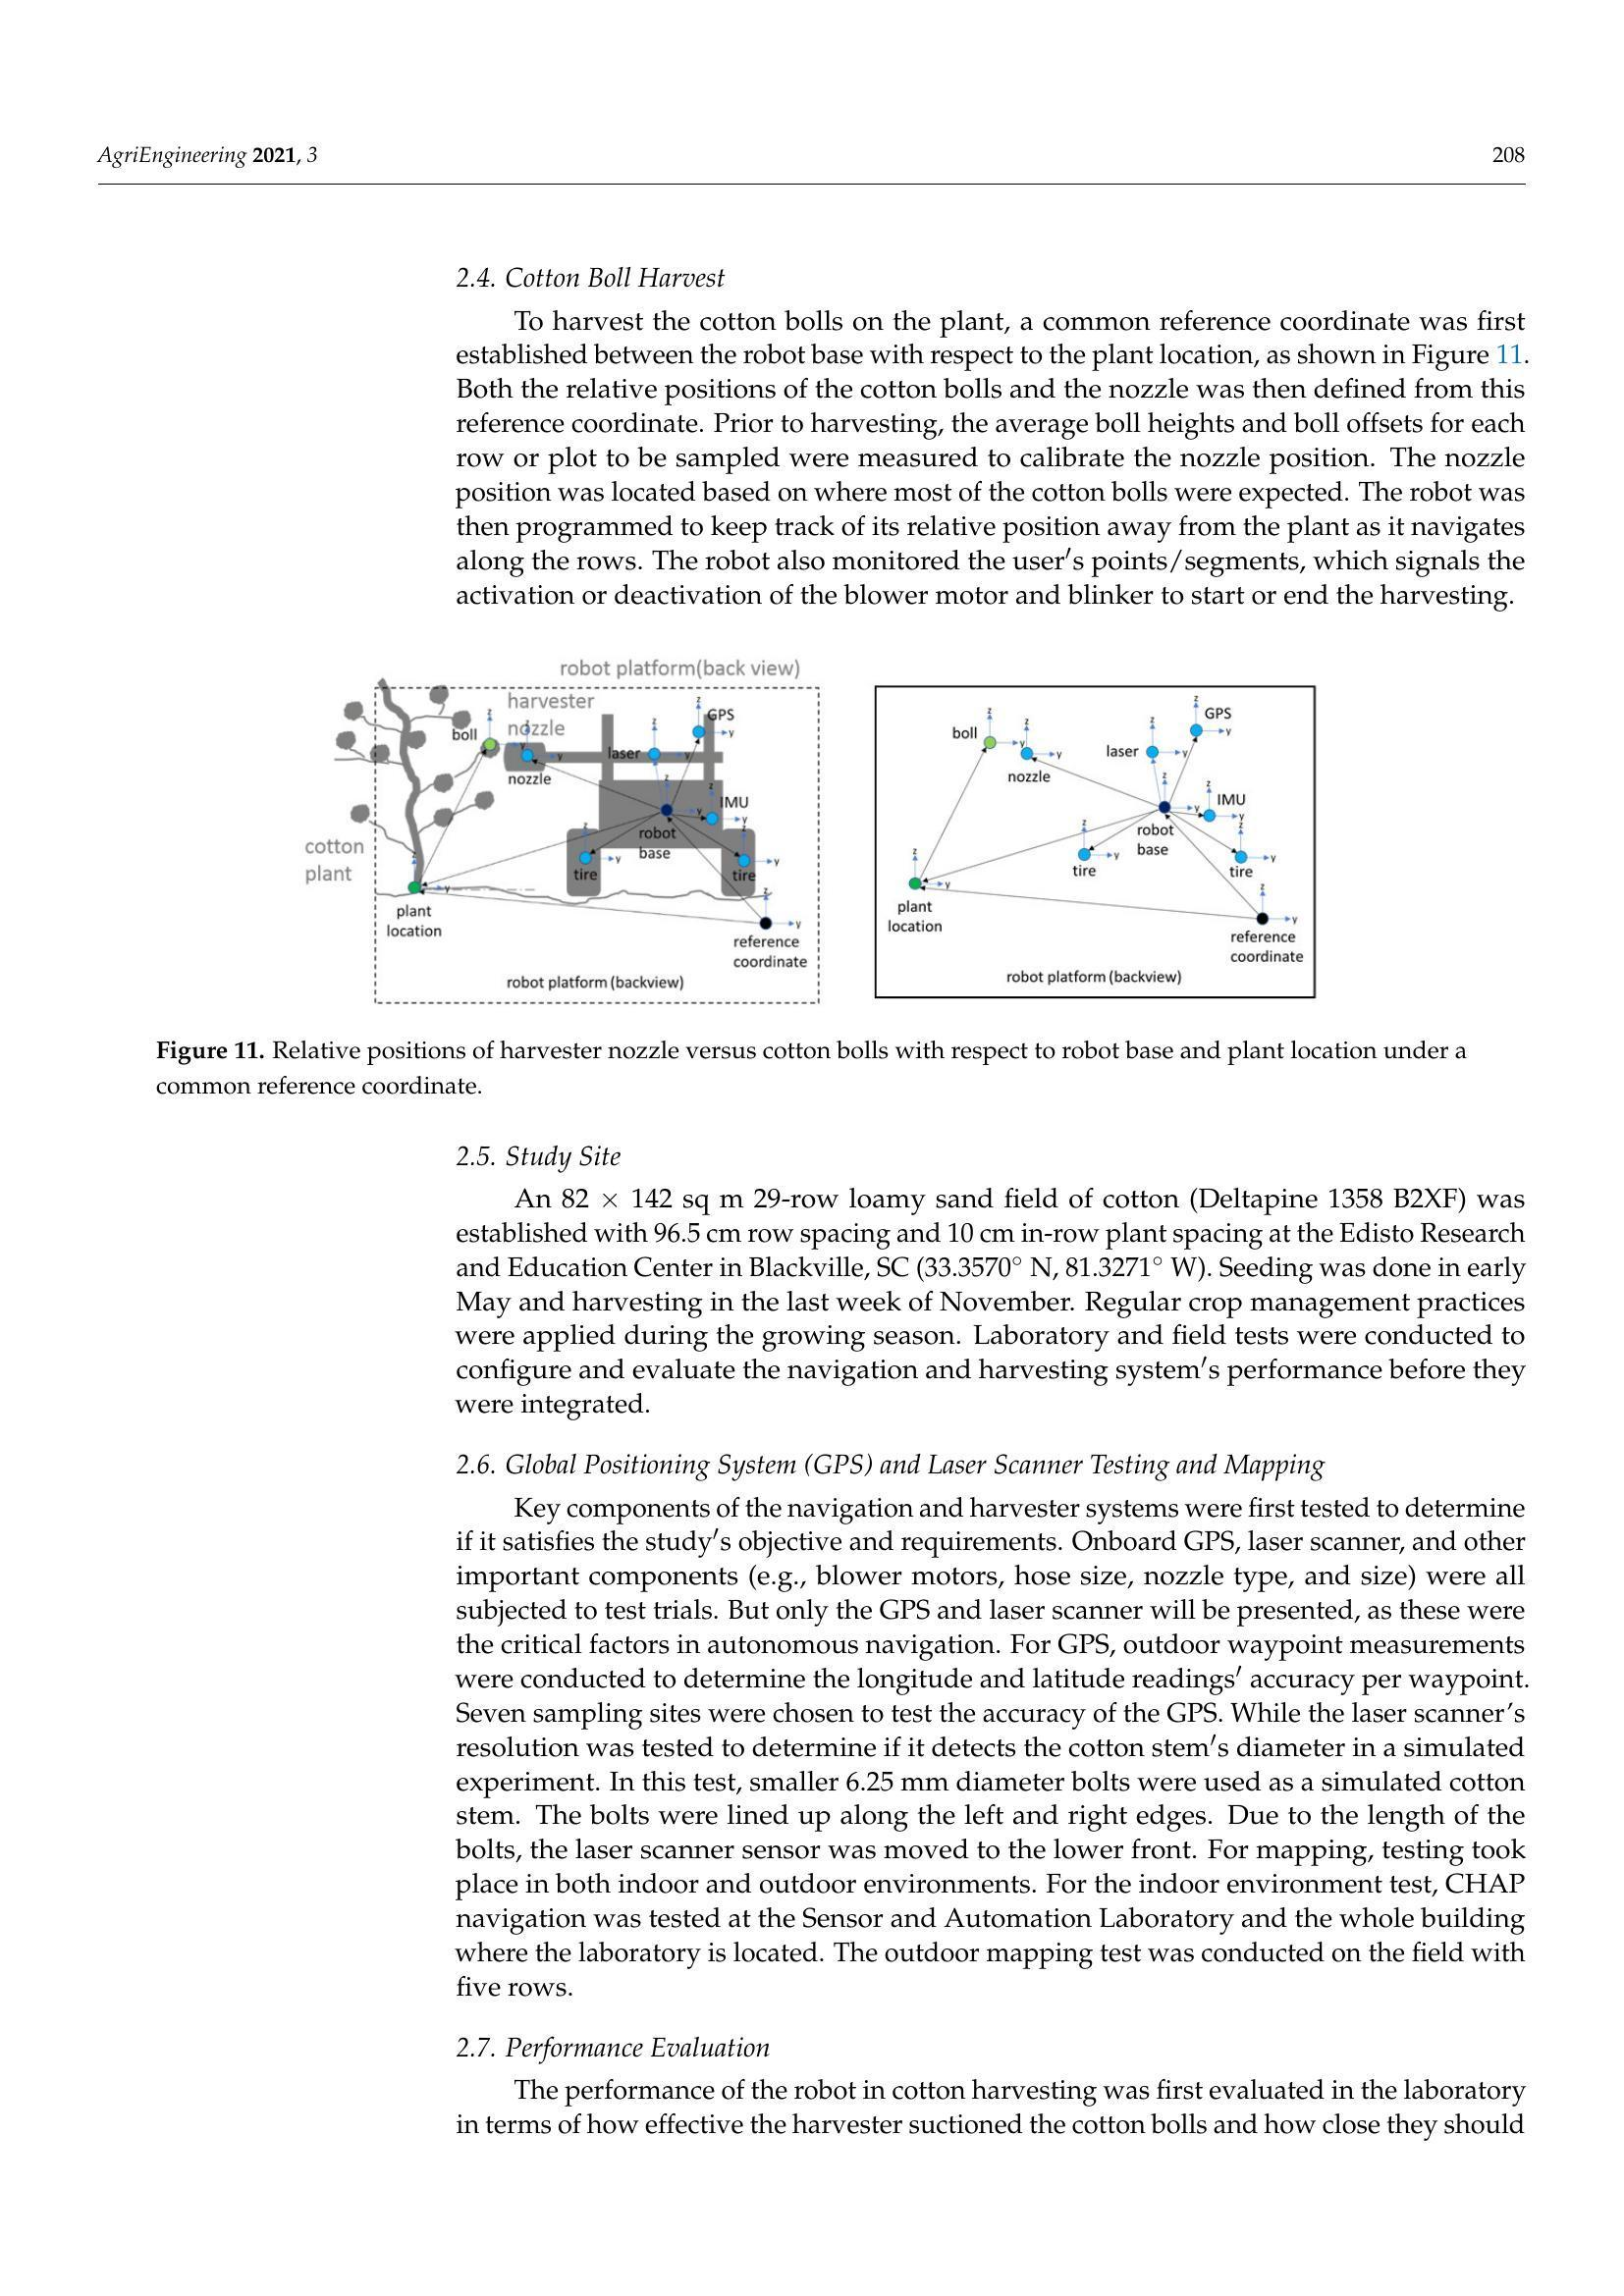
\includegraphics[width=\textwidth]{images/colpali_images/dataset_samples/ai_2.jpeg}
        \end{subfigure} \ 
        \begin{subfigure}[t]{0.30\textwidth}
            \caption*{\textbf{Query}: What is the key approach used in the PDP architecture?}
            \includegraphics*[width=\textwidth]{images/colpali_images/dataset_samples/ai_3.jpeg}
        \end{subfigure}
    \end{figure}

    \newpage
    \vspace*{3\baselineskip}

    \textbf{Healthcare Industry} \\[1ex]
    \begin{figure}[h]
        \centering
        \begin{subfigure}[t]{0.30\textwidth}
            \caption*{\textbf{Query}: What is the chemical formula for the ferroelectric material Lead Zirconium Titanate (PZT)?}
            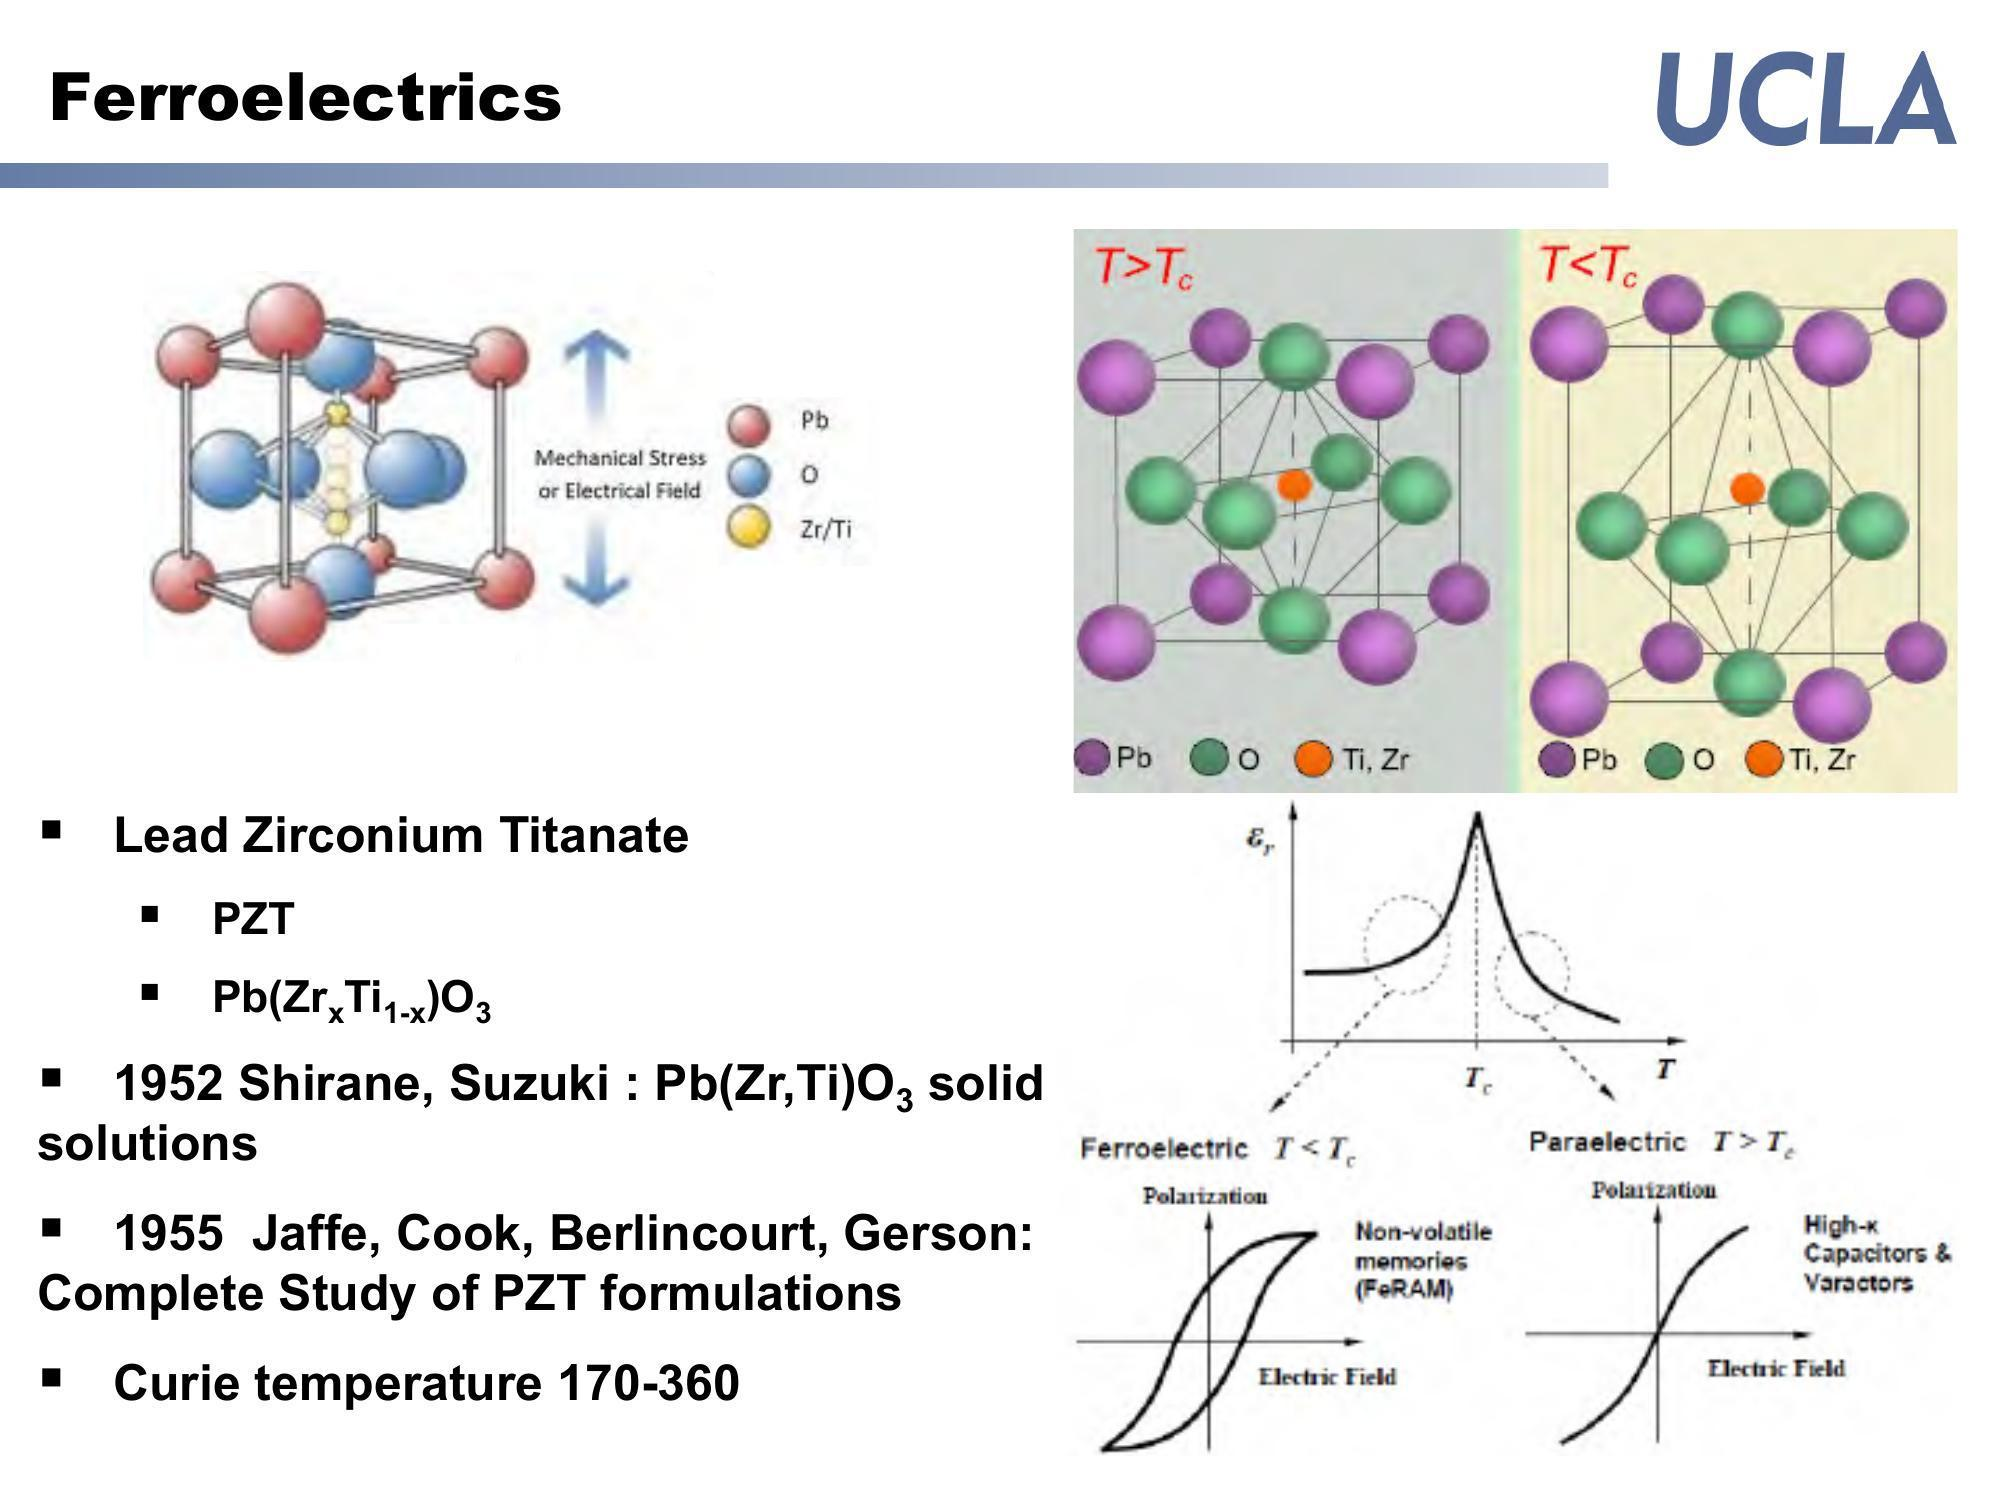
\includegraphics[width=\textwidth]{images/colpali_images/dataset_samples/healthcare_1.jpeg}
        \end{subfigure} \ 
        \begin{subfigure}[t]{0.30\textwidth}
            \caption*{\textbf{Query}: What government entities are involved in public financing for healthcare in the US?}
            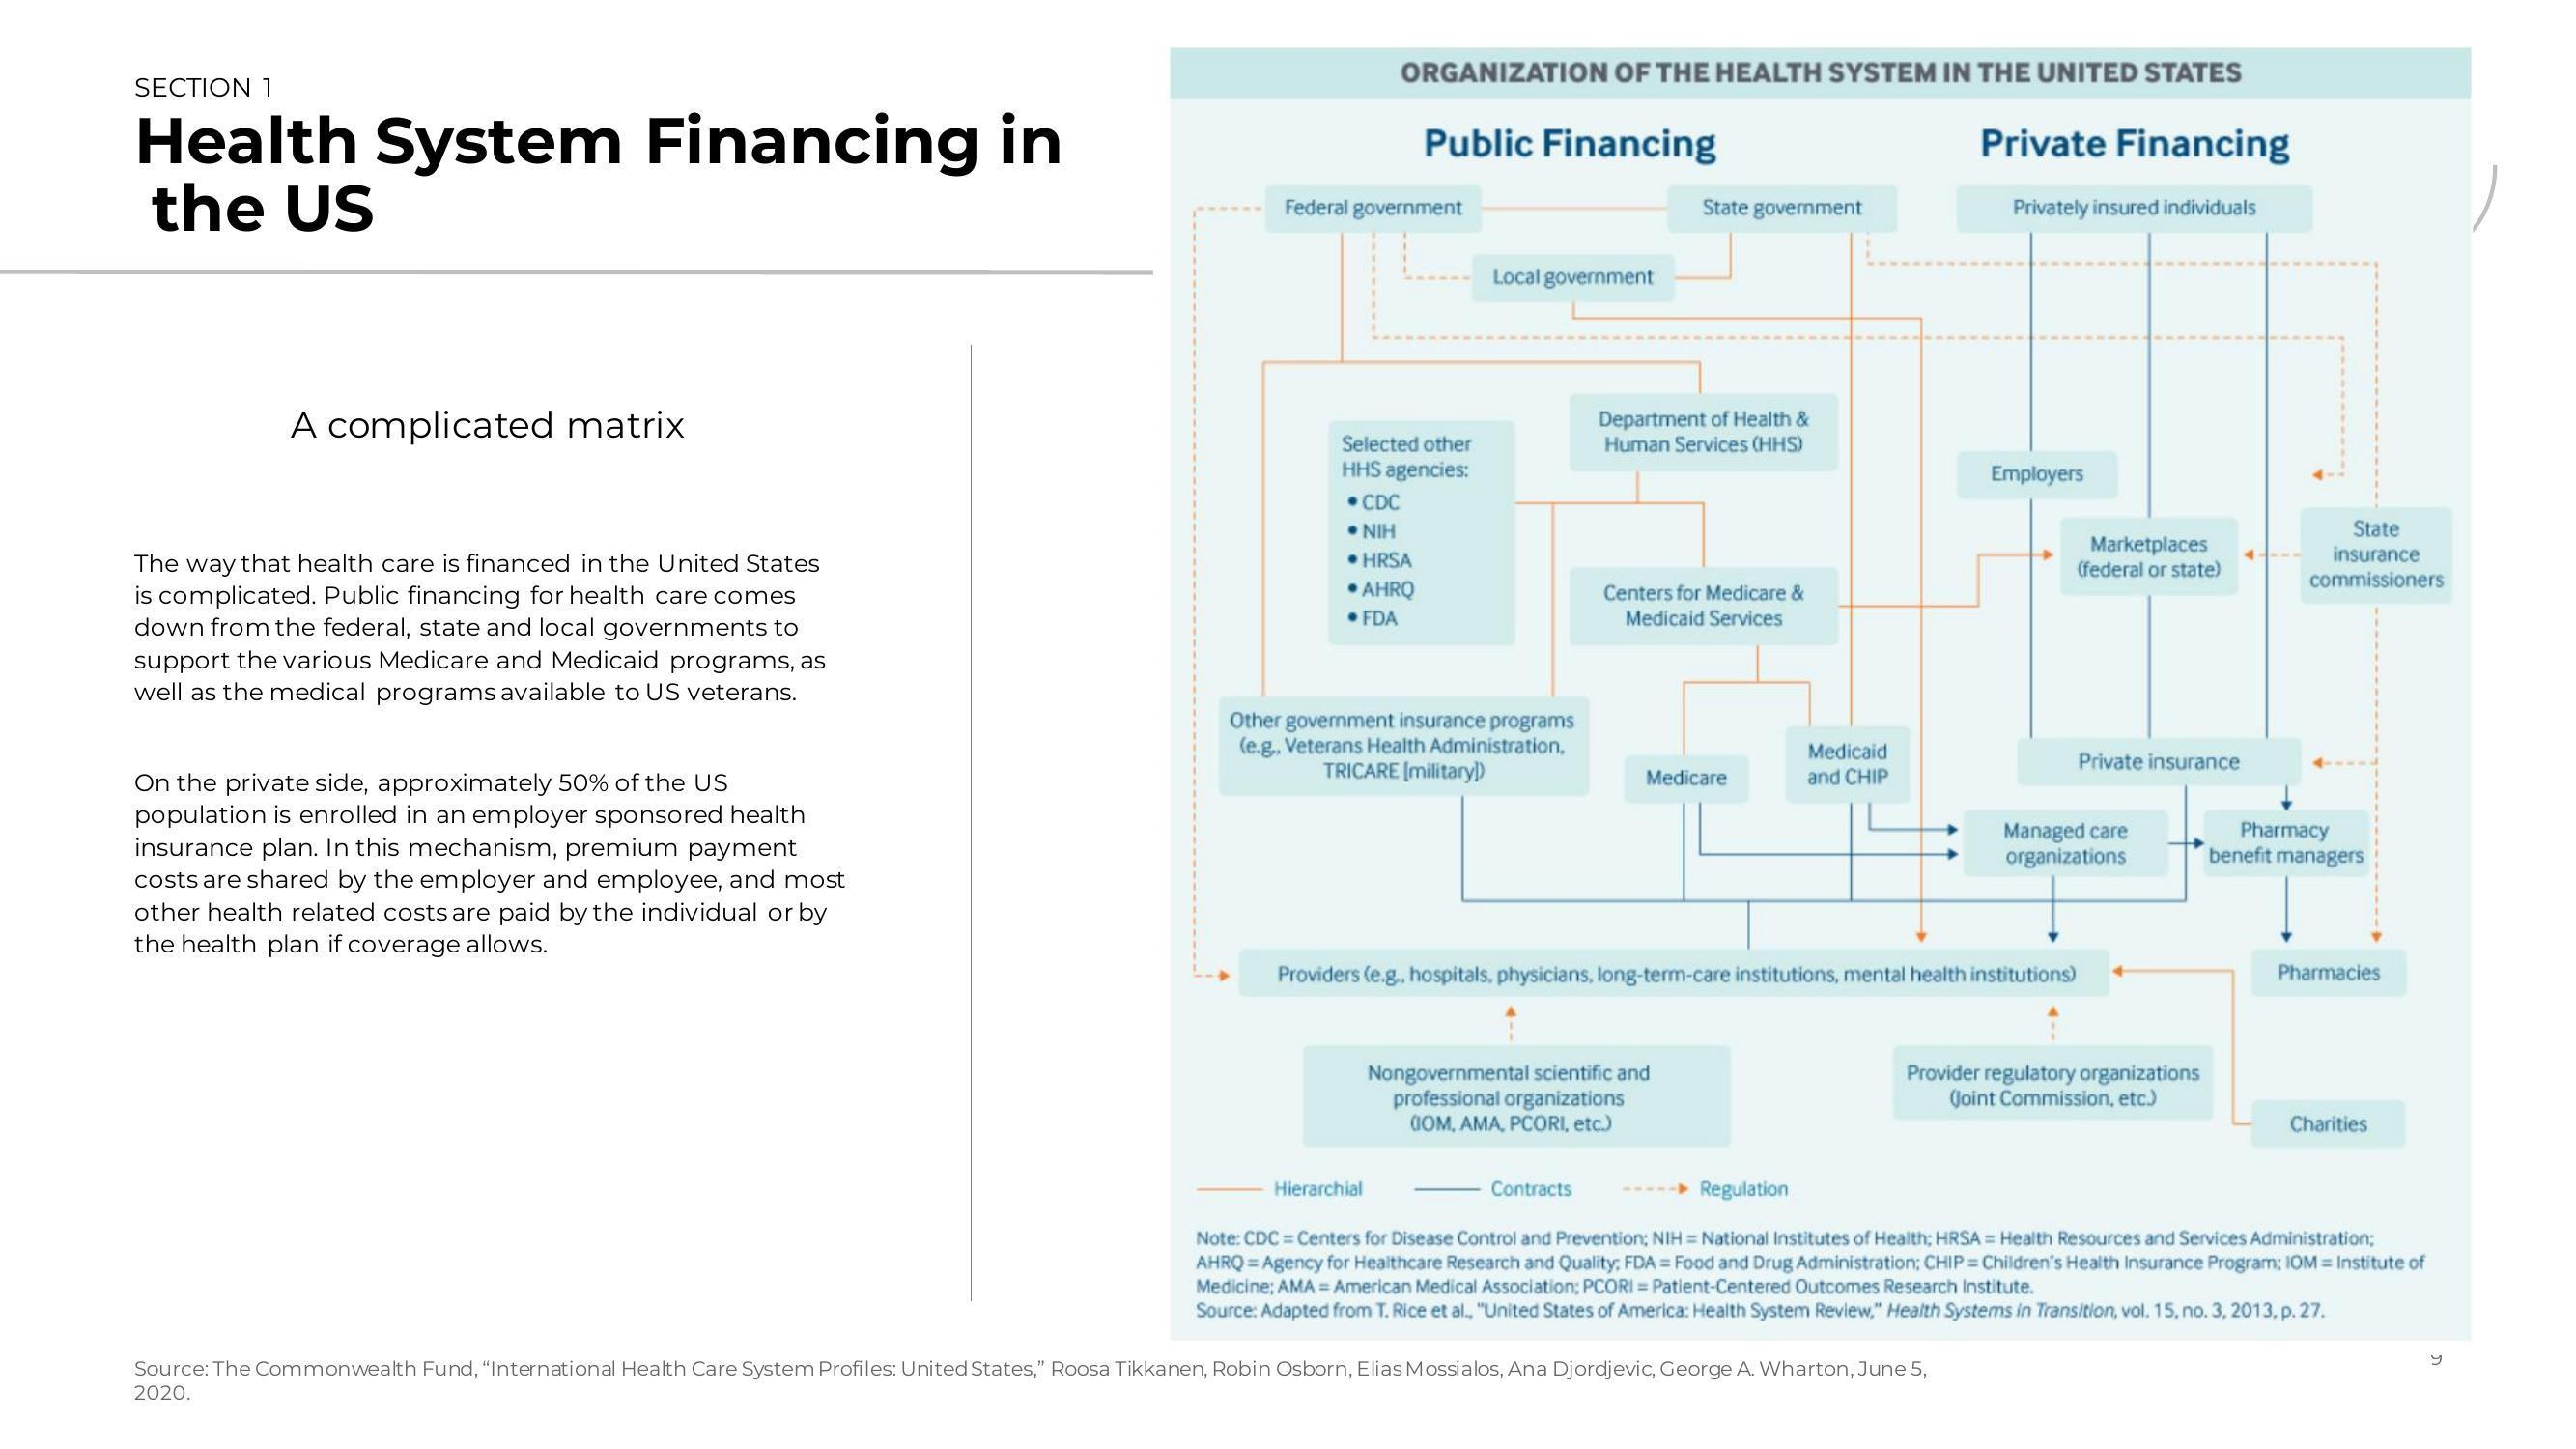
\includegraphics[width=\textwidth]{images/colpali_images/dataset_samples/healthcare_2.jpeg}
        \end{subfigure} \ 
        \begin{subfigure}[t]{0.30\textwidth}
            \caption*{\textbf{Query}: What does the AVPU scale stand for in assessing the level of consciousness of a seriously ill child?}
            \includegraphics*[width=\textwidth]{images/colpali_images/dataset_samples/healthcare_3.jpeg}
        \end{subfigure}
    \end{figure}

    \vspace*{5\baselineskip}

    \textbf{Government Reports} \\[1ex]
    \begin{figure}[h]
        \centering
        \begin{subfigure}[t]{0.30\textwidth}
            \caption*{\textbf{Query}: What are some mandates for the EPA under the Pollution Prevention Act?}
            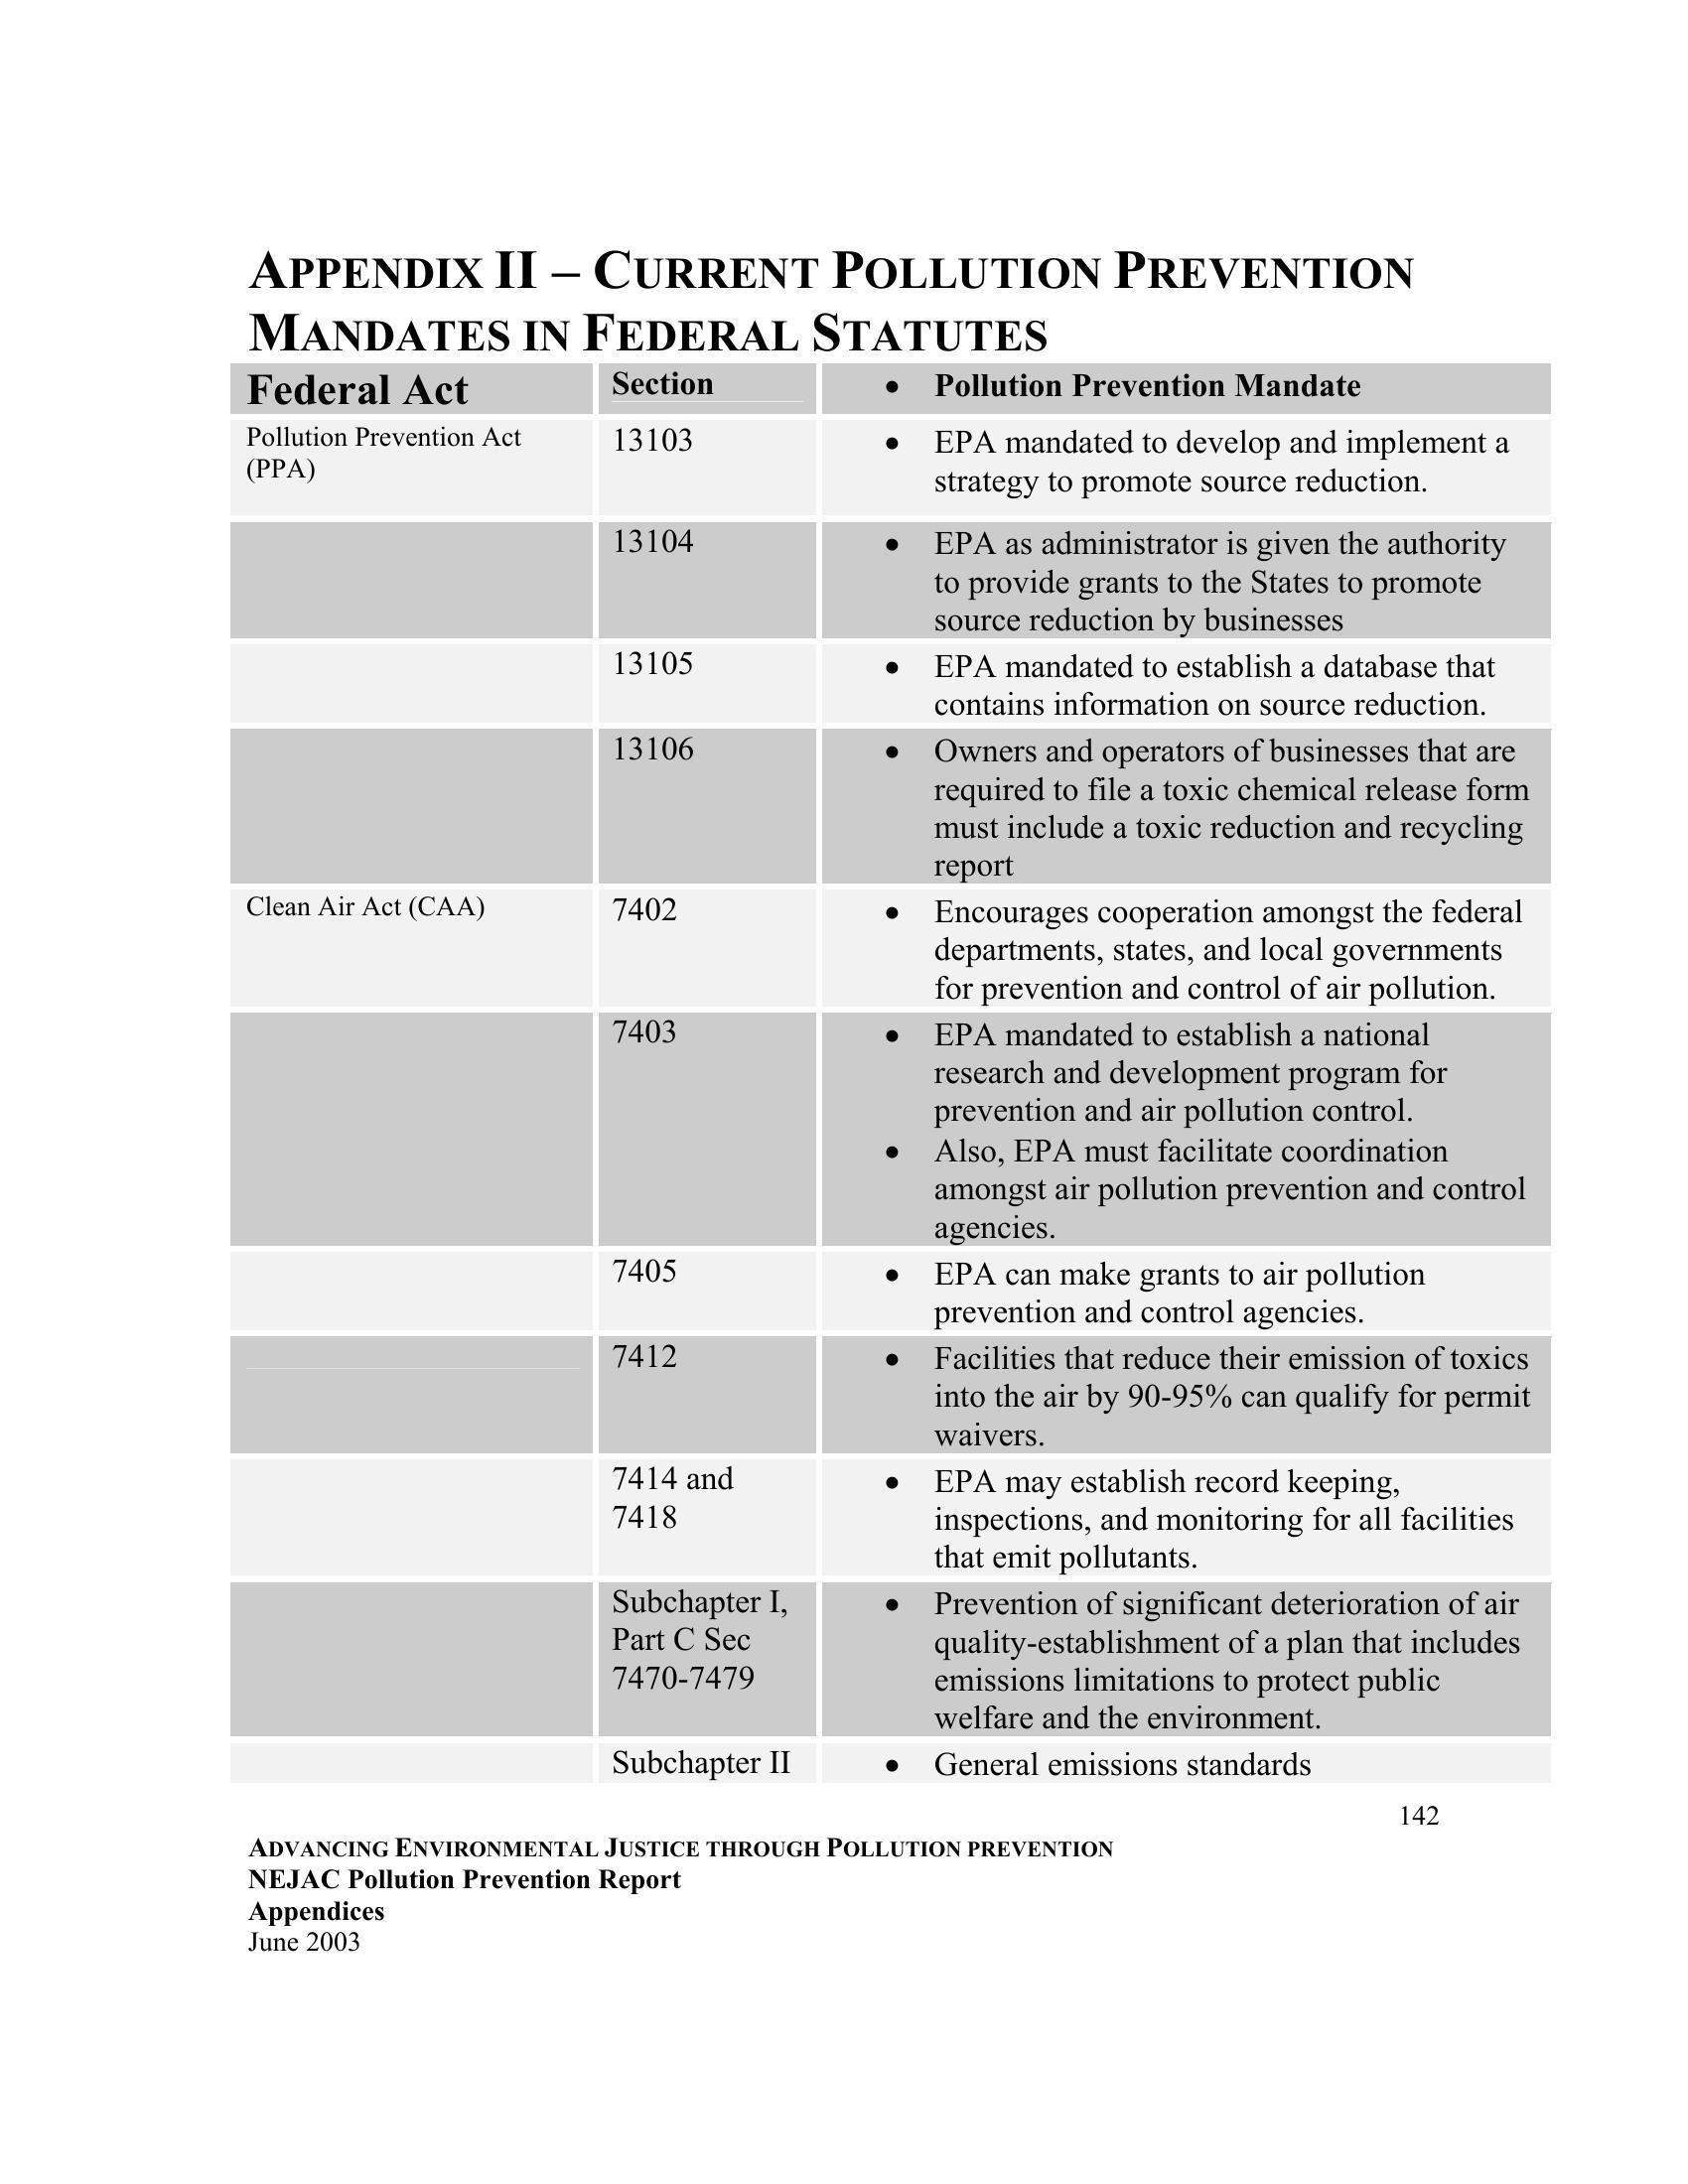
\includegraphics[width=\textwidth]{images/colpali_images/dataset_samples/gov_1.jpeg}
        \end{subfigure} \ 
        \begin{subfigure}[t]{0.30\textwidth}
            \caption*{\textbf{Query}: What is the strategy of KPMG Hazem Hassan?}
            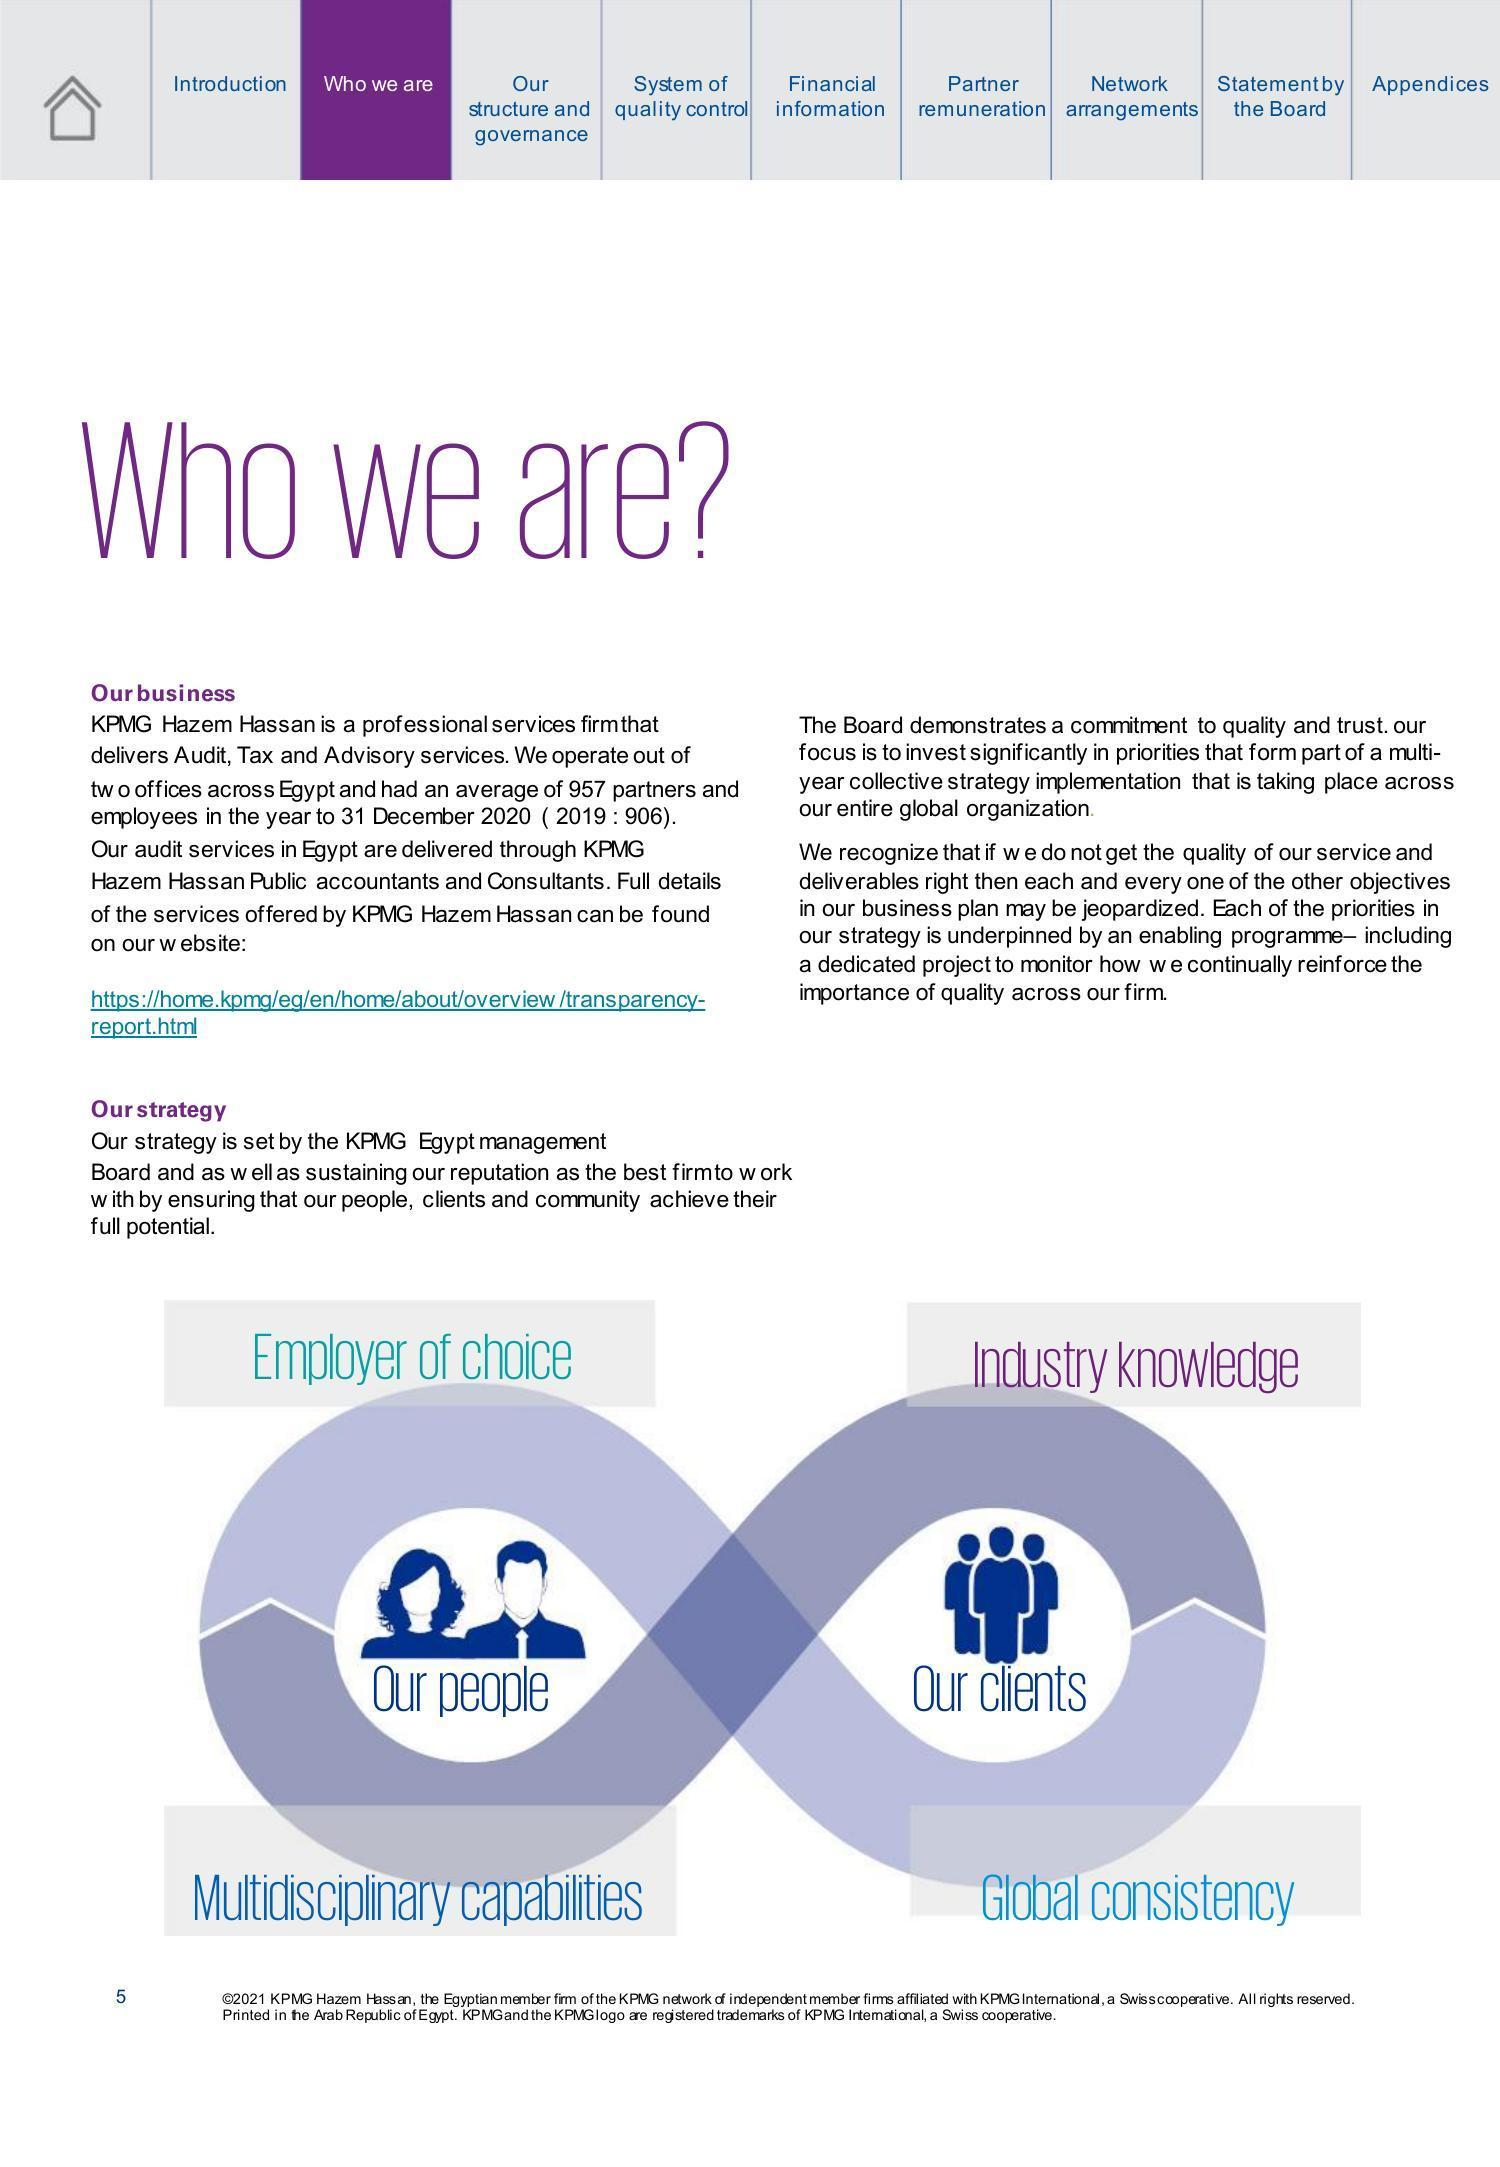
\includegraphics[width=\textwidth]{images/colpali_images/dataset_samples/gov_2.jpeg}
        \end{subfigure} \ 
        \begin{subfigure}[t]{0.30\textwidth}
            \caption*{\textbf{Query}: What is the trust signal score for the consumer industry best-in-class archetype?}
            \includegraphics*[width=\textwidth]{images/colpali_images/dataset_samples/gov_3.jpeg}
        \end{subfigure}
    \end{figure}

    \newpage
    \vspace*{3\baselineskip}

    \textbf{Shift} \\[1ex]
    \begin{figure}[h]
        \centering
        \begin{subfigure}[t]{0.30\textwidth}
            \caption*{\textbf{Query}: Selon le graphique, quelle est la capacité d'import et la consommation réelle de carburants SAF (biocarburants durables pour l'aviation) prévues en 2050 ?}
            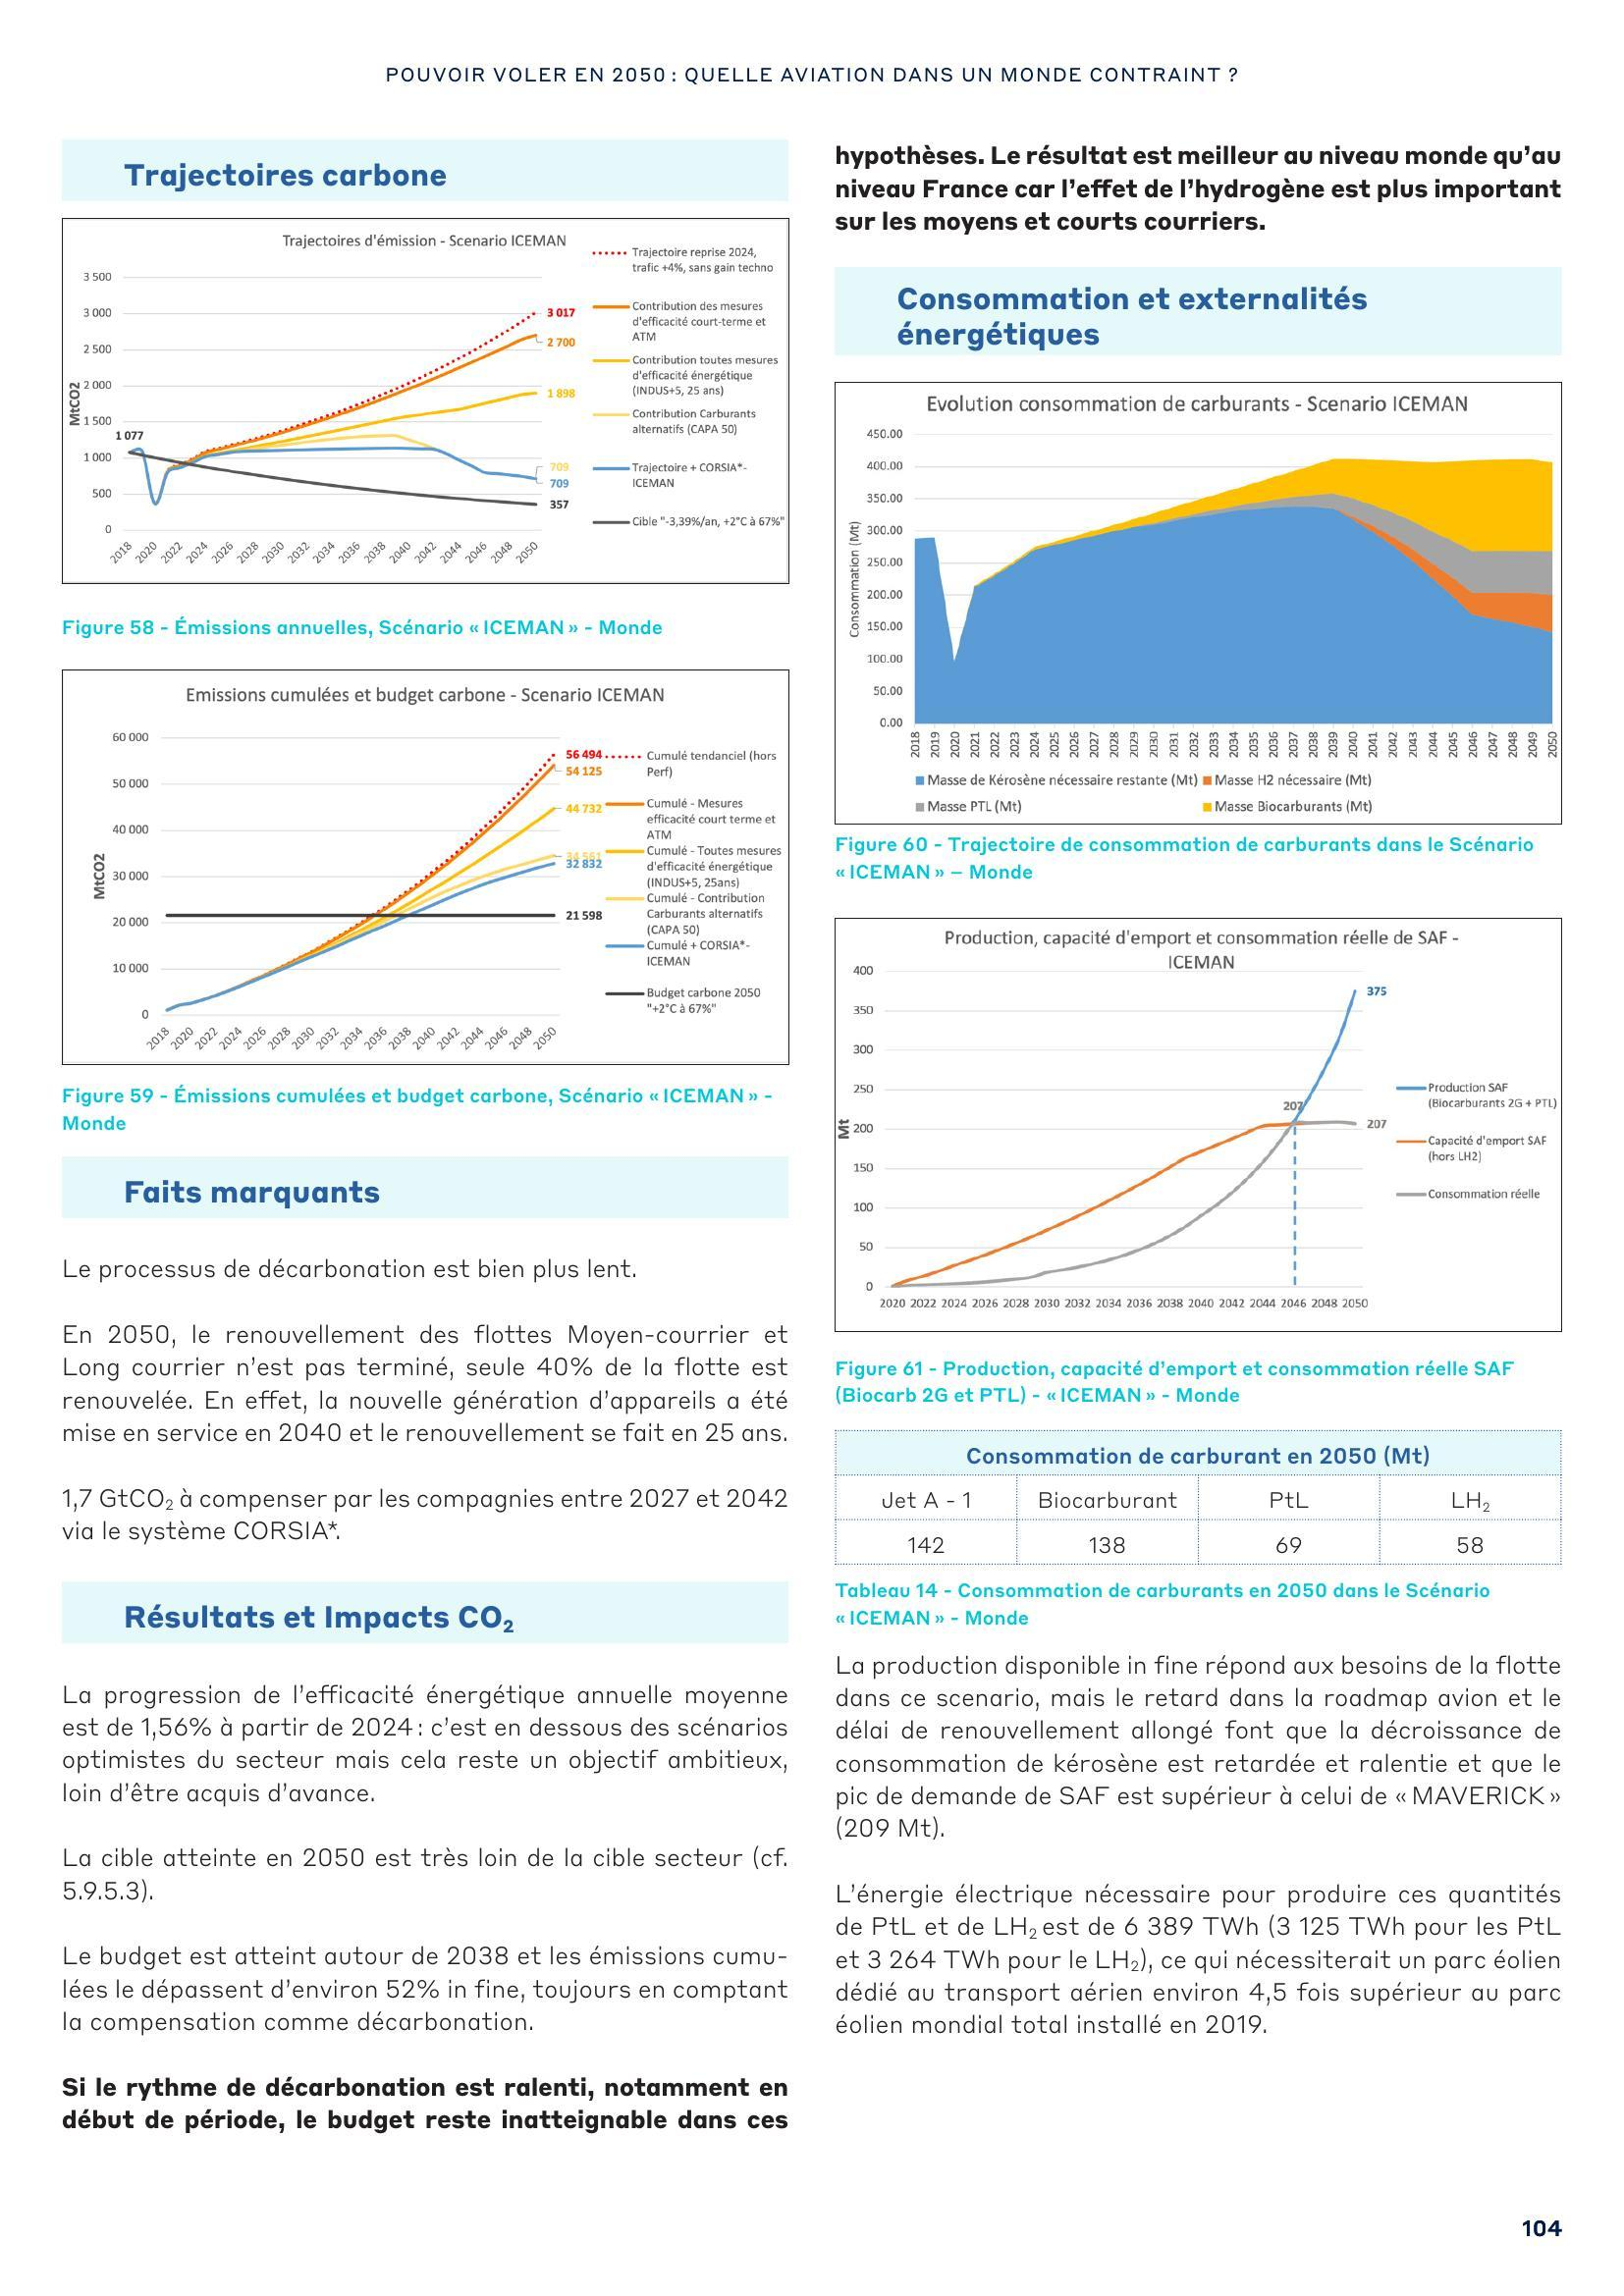
\includegraphics[width=\textwidth]{images/colpali_images/dataset_samples/shift_1.jpeg}
        \end{subfigure} \ 
        \begin{subfigure}[t]{0.30\textwidth}
            \caption*{\textbf{Query}: Quelle partie de la production pétrolière du Kazakhstan provient de champs en mer ?}
            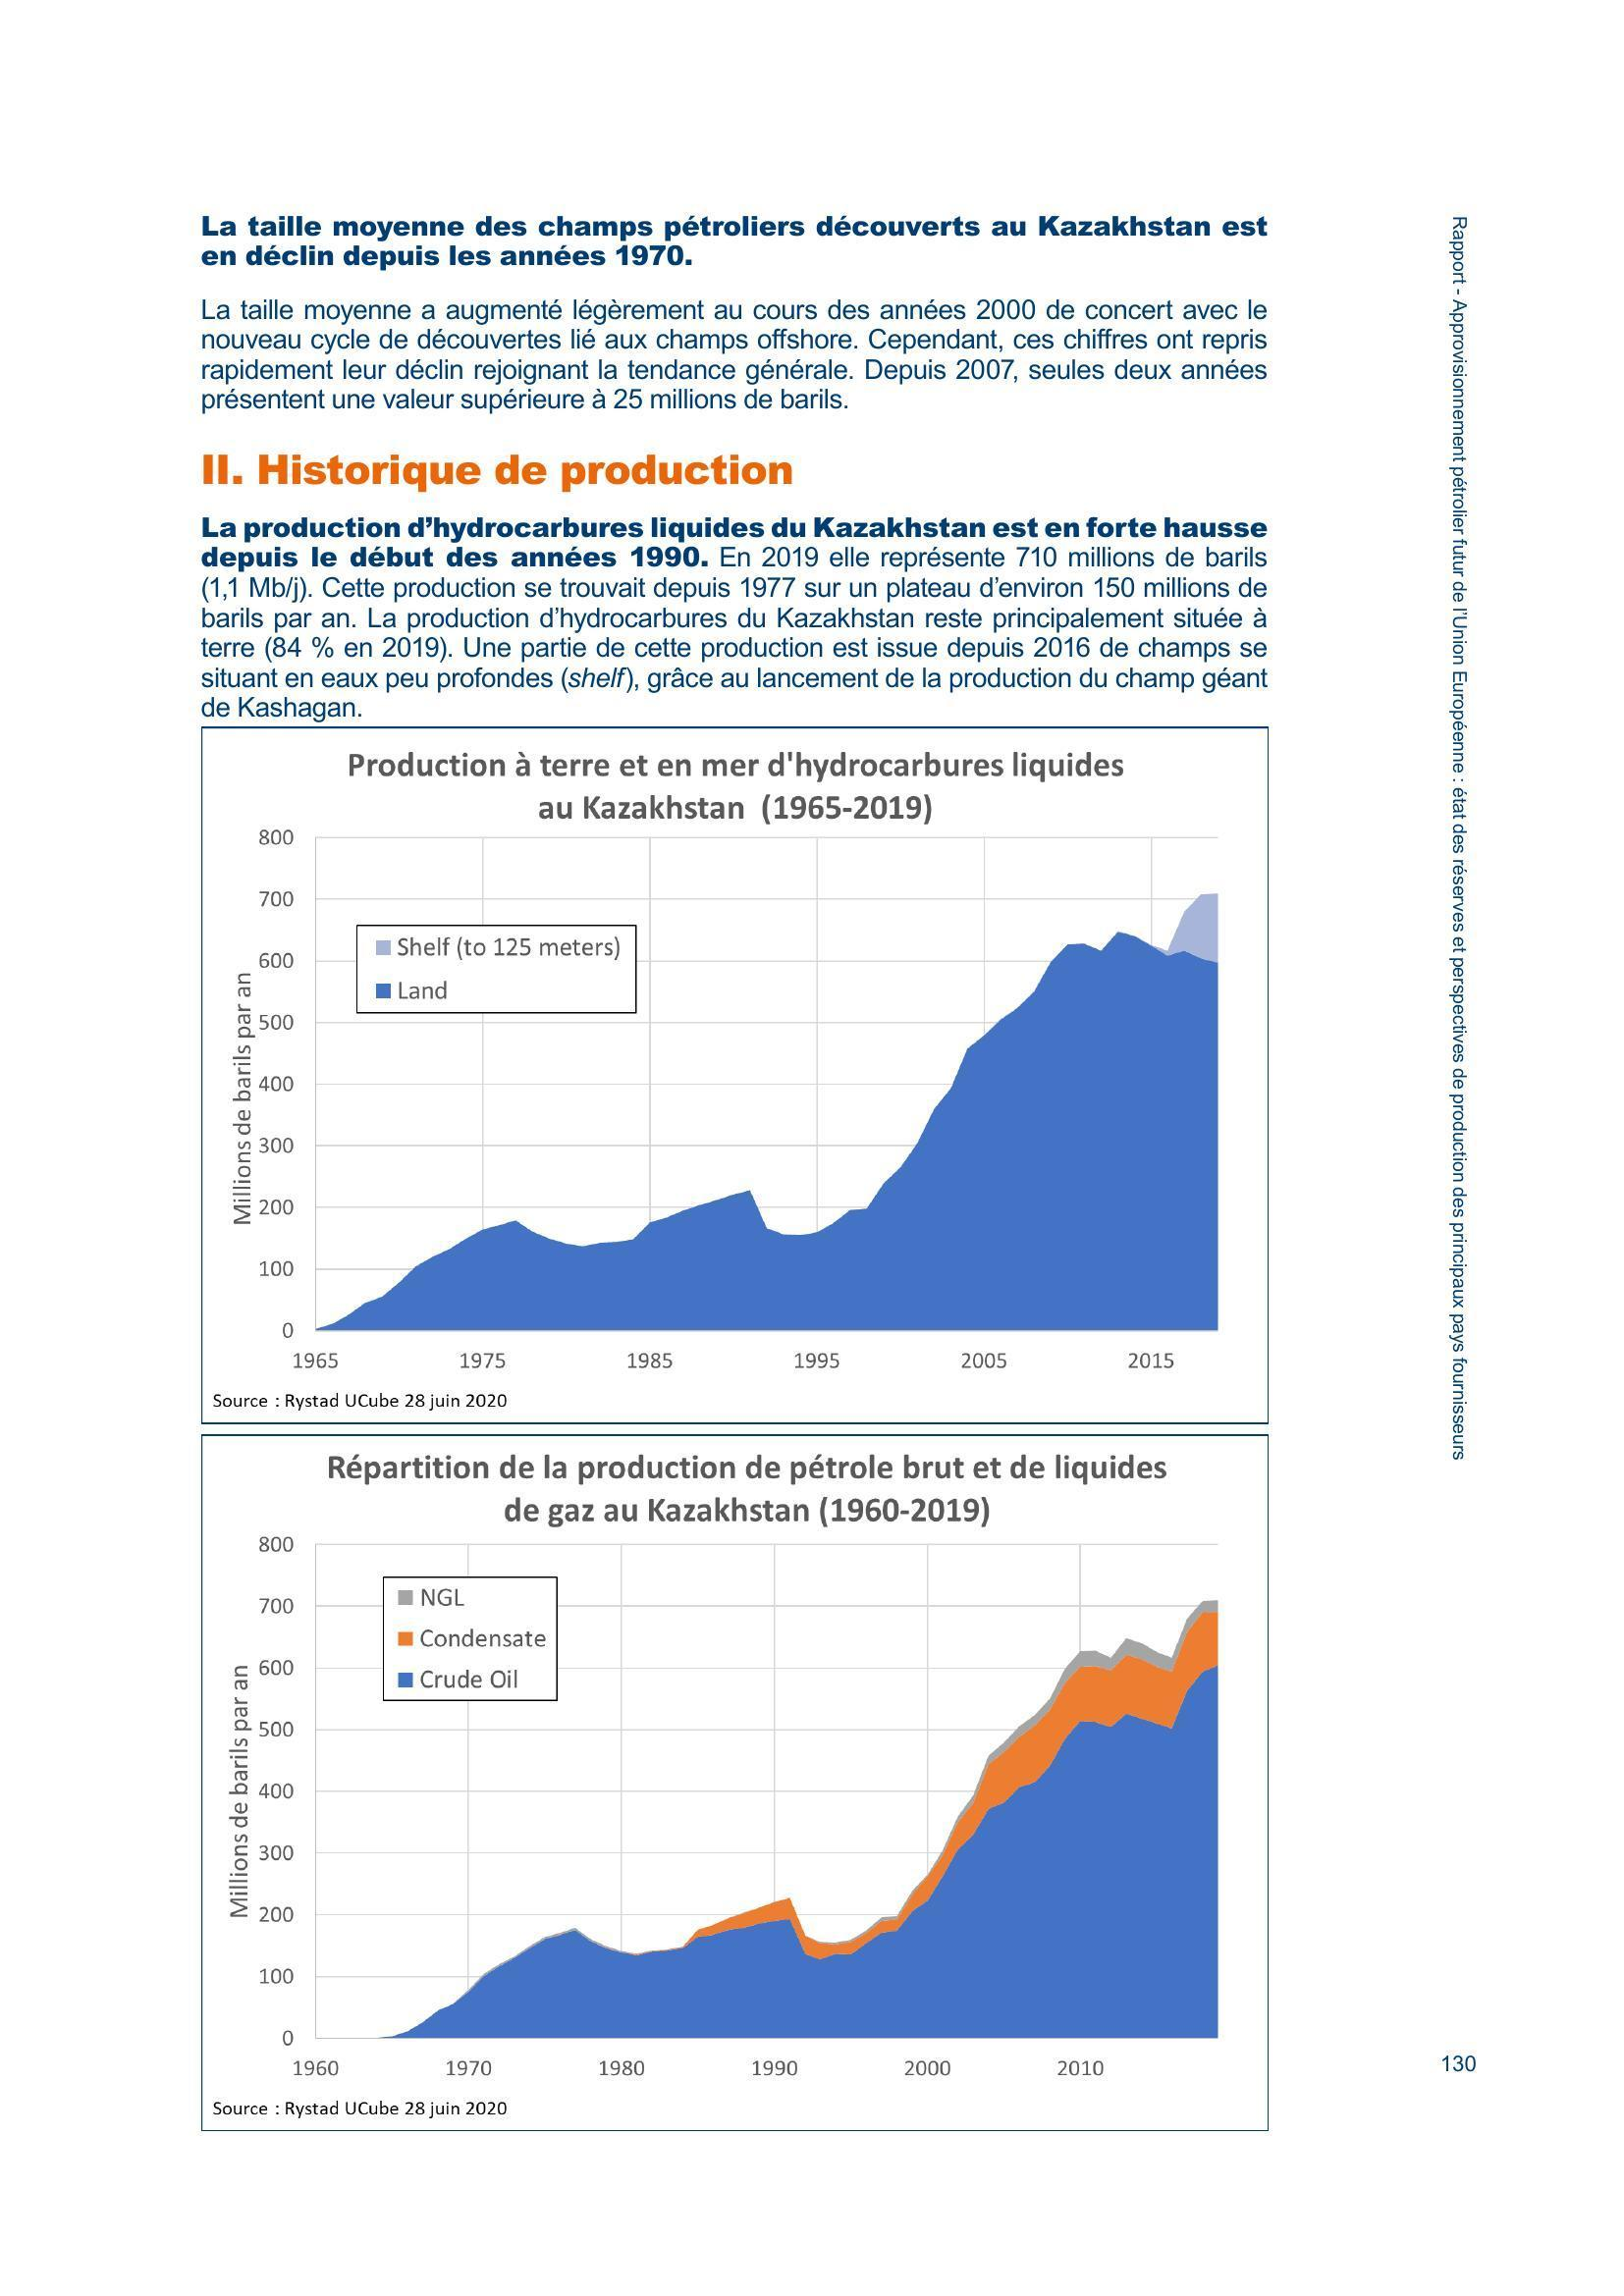
\includegraphics[width=\textwidth]{images/colpali_images/dataset_samples/shift_2.jpeg}
        \end{subfigure} \ 
        \begin{subfigure}[t]{0.30\textwidth}
            \caption*{\textbf{Query}: Quels sont les pays ayant la plus grande part des découvertes cumulées de pétrole brut en 2020 (en milliers de barils, hors découvertes cumulées) ?}
            \includegraphics*[width=\textwidth]{images/colpali_images/dataset_samples/shift_3.jpeg}
        \end{subfigure}modelsmodels
    \end{figure}

\end{center}
